\documentclass[UTF8,a4paper,12pt]{ctexart}

% 全文版式统一采用杨昊东学位论文的可见结构体系
% 杨昊东论文可见版式的LaTeX统一样式层
% 目标：章节、图表、公式、目录、摘要、参考文献等版式与参考论文保持同一体系。
% 说明：学校封面中的姓名、导师、专业等个体信息不在此文件中硬编码。

\usepackage{amsmath,amssymb,graphicx,booktabs,multirow}
\usepackage{geometry}
\usepackage{caption}
\usepackage{fancyhdr}
\usepackage{chngcntr}
\usepackage{setspace}
\usepackage{indentfirst}
\usepackage{titlesec}
\usepackage{tocloft}
\usepackage{hyperref}
\usepackage{etoolbox}

% A4学位论文正文版心。以参考论文的Word学位论文版式为基准统一。
\geometry{a4paper,top=2.54cm,bottom=2.54cm,left=3.00cm,right=2.60cm,headheight=14pt,headsep=0.60cm,footskip=1.20cm}

% 正文字体与段落
\zihao{-4}
\setstretch{1.5}
\setlength{\parindent}{2em}
\setlength{\parskip}{0pt}

% 将ctexart的一级section作为“章”使用：第一章、第二章……
\ctexset{
  section = {
    name = {第,章},
    number = \chinese{section},
    format = \centering\heiti\zihao{3},
    beforeskip = 0pt,
    afterskip = 1.2\baselineskip
  },
  subsection = {
    format = \heiti\zihao{-3},
    beforeskip = 0.8\baselineskip,
    afterskip = 0.4\baselineskip
  },
  subsubsection = {
    format = \heiti\zihao{4},
    beforeskip = 0.6\baselineskip,
    afterskip = 0.3\baselineskip
  }
}

% 每章另起一页；首章也如此
\pretocmd{\section}{\clearpage}{}{}

% 节标题按1.1、1.1.1编号
\renewcommand{\thesubsection}{\arabic{section}.\arabic{subsection}}
\renewcommand{\thesubsubsection}{\arabic{section}.\arabic{subsection}.\arabic{subsubsection}}

% 图、表、公式按章编号：图2-1、表2-1、式(2-1)
\counterwithin{figure}{section}
\counterwithin{table}{section}
\numberwithin{equation}{section}
\renewcommand{\thefigure}{\arabic{section}-\arabic{figure}}
\renewcommand{\thetable}{\arabic{section}-\arabic{table}}
\renewcommand{\theequation}{\arabic{section}-\arabic{equation}}
\renewcommand{\figurename}{图}
\renewcommand{\tablename}{表}

% 图表题注居中，题注字号统一
\captionsetup{font={small},labelsep=space,justification=centering,singlelinecheck=true}
\captionsetup[table]{position=top,skip=6pt}
\captionsetup[figure]{position=bottom,skip=6pt}

% 页眉页脚：正文保持学位论文简洁形式
\pagestyle{fancy}
\fancyhf{}
\fancyfoot[C]{\thepage}
\renewcommand{\headrulewidth}{0pt}
\renewcommand{\footrulewidth}{0pt}

% 目录：列至三级标题，与参考论文目录层级一致
\setcounter{tocdepth}{3}
\renewcommand{\contentsname}{目录}
\renewcommand{\cftsecfont}{\songti}
\renewcommand{\cftsubsecfont}{\songti}
\renewcommand{\cftsubsubsecfont}{\songti}
\renewcommand{\cftsecpagefont}{\songti}
\renewcommand{\cftsubsecpagefont}{\songti}
\renewcommand{\cftsubsubsecpagefont}{\songti}

% 超链接仅保留PDF内部跳转，不出现彩色框线
\hypersetup{hidelinks,unicode=true}

% 摘要页标题命令
\newcommand{\cnabstracttitle}{%
  \begin{center}\heiti\zihao{3} 摘\quad 要\end{center}\vspace{0.8\baselineskip}}
\newcommand{\enabstracttitle}{%
  \begin{center}\bfseries\zihao{3} Abstract\end{center}\vspace{0.8\baselineskip}}

% 关键词格式
\newcommand{\cnkeywords}[1]{\par\vspace{0.8\baselineskip}\noindent\textbf{关键词：}#1}
\newcommand{\enkeywords}[1]{\par\vspace{0.8\baselineskip}\noindent\textbf{Keywords: }#1}

% 参考文献标题和目录入口
\renewcommand{\refname}{参考文献}
\newcommand{\printthesisbibliography}{%
  \clearpage
  \phantomsection
  \addcontentsline{toc}{section}{参考文献}
  \bibliographystyle{gbt7714-numerical}
  \bibliography{references/publication,references/methods,references/local_theses,references/kg_sources}
}

% 最终图文件由SVG在编译前统一转换为PDF；旧章节中的.svg引用透明映射到同名PDF。
% Final-stage figure bridge.
% build_thesis.sh converts all tracked SVG figures to sibling PDF files before XeLaTeX.
% This graphics rule lets legacy \includegraphics{...svg} calls transparently load the converted PDF.
\DeclareGraphicsRule{.svg}{pdf}{.pdf}{}


\begin{document}

% 当前仓库暂不写入学校、姓名、导师等个人封面字段，避免编造信息。
% 后续可在不改正文的情况下单独增加封面页。

% -------------------- 前置部分 --------------------
\pagenumbering{Roman}
\setcounter{page}{1}

\phantomsection
\addcontentsline{toc}{section}{摘要}
\cnabstracttitle

在新能源高比例并网和煤电机组深度调峰背景下，燃煤机组汽轮机长期处于宽负荷、频繁变工况运行状态，其压力、温度、流量等热工参数不仅受设备健康状态影响，还随负荷水平、蒸汽边界及运行调节持续变化。同时，汽轮机系统具有明显的多设备、多参数耦合特征，而现场高质量故障样本数量有限，传统固定阈值及单纯依赖故障样本的数据驱动方法难以兼顾变工况适应性、故障识别精度和诊断解释性。本文以燃煤机组汽轮机热力系统为研究对象，围绕设备健康状态监测、故障知识图谱构建及KG-GCN故障诊断方法开展研究。主要研究内容包括：

针对汽轮机正常运行参数随工况变化而持续迁移、固定设计基准难以直接用于长期状态评价的问题，提出基于GRU的设备级健康状态监测方法。该方法依据设备实际热力边界，将操作变量和上游/外部边界作为输入，以设备本体及接口状态参数作为输出，通过时序模型学习给定运行条件下的健康响应关系。以超高压缸（VHP）为代表性对象，采用2024年5月正常DCS数据训练模型，并以2024年6月数据进行独立测试，同时设置ANN、TCN和iTransformer-small进行对比。结果表明，GRU在最终24个状态参数上的宏平均$R^2$达到0.9511，在VHP本体、一级抽汽及一次冷再接口等主要状态上均能够形成较稳定的动态健康参考，为后续利用实测值与健康预测值之间的偏差表征设备状态变化提供了基础。

针对汽轮机设备关系复杂、故障知识分散于DCS点表、设备结构资料及故障文献中的问题，构建基于运行生产资料的汽轮机系统故障知识图谱。根据汽轮机主通流、再热、抽汽回热及凝汽冷端等实际热力过程，定义设备、参数、异常、故障和处置等实体类型以及相应关系类型；采用大语言模型生成候选三元组，并结合实体类型规则、关系方向、本机设备兼容性、来源证据及Embedding语义对齐完成知识校核和实体标准化。当前审计知识库包含127个标准实体和123条候选关系，其中121条关系进入主知识图谱，2条存在资料差异的候选关系保留待核。由此将分散的设备结构信息与故障机理转化为可用于图卷积计算的结构化领域知识。

针对不同汽轮机故障可能共享局部监测参数以及故障标签数量有限的问题，提出基于知识图谱与图卷积网络的KG-GCN故障诊断方法。该方法将健康状态模型产生的多参数残差按时间窗口映射为知识图谱参数节点的动态特征，并将知识图谱投影得到的参数关系作为图结构输入，通过GCN沿设备和参数关联关系逐层聚合故障特征。训练阶段首先在不使用类别标签的残差窗口上进行随机遮蔽重构预训练，随后固定图卷积编码器并利用带标签故障窗口训练分类层。以VHP为代表性算例，基于真实健康运行残差和独立故障机理构造正常状态、VHP通流部件侵蚀、一级抽汽支路泄漏和VHP汽封泄漏四类半物理诊断场景。固定随机种子实验中，KG-GCN的诊断Accuracy和F1分别达到98.57\%和98.58\%，优于CNN和AE；3组随机种子重复实验的平均Macro-F1达到98.46\%$\pm$0.11\%。在分类阶段仅使用20\%带标签故障窗口时，掩码预训练使Macro-F1由94.48\%提高至96.67\%，表明知识拓扑与残差预训练能够在故障标签有限条件下提高诊断性能和结果稳定性。

综上，本文形成了由“设备健康状态建模—动态状态残差—汽轮机故障知识图谱—图卷积特征聚合—掩码预训练—故障分类”组成的汽轮机系统状态监测与故障诊断流程。本文故障分类实验采用真实健康残差背景与独立机理构造的半物理故障场景，相关结果验证了所提方法在当前代表性算例中的有效性；其面向现场真实故障及其他汽轮机设备的工程泛化能力仍需结合后续故障记录和经实测数据校准的仿真样本进一步验证。

\cnkeywords{燃煤机组；汽轮机系统；状态监测；知识图谱；图卷积网络；故障诊断}

\clearpage
\phantomsection
\addcontentsline{toc}{section}{Abstract}
\enabstracttitle

With the increasing penetration of renewable energy and the deep peak-regulation operation of coal-fired power units, steam turbine systems are increasingly operated under wide-load and frequently varying conditions. Their pressure, temperature and flow parameters are affected not only by equipment health conditions, but also by unit load, steam boundaries and operating adjustments. Meanwhile, the steam turbine system exhibits strong coupling among multiple devices and parameters, whereas high-quality field fault samples are scarce. Consequently, conventional fixed-threshold methods and purely data-driven methods relying on labeled fault samples have difficulty simultaneously achieving adaptability to varying operating conditions, accurate fault identification and diagnostic interpretability. This thesis takes the thermal system of a coal-fired steam turbine as the research object and investigates equipment health condition monitoring, fault knowledge graph construction and KG-GCN-based fault diagnosis. The main research contents are as follows.

To address the continuous migration of normal steam turbine parameters with operating conditions, which makes a fixed design reference unsuitable for long-term condition assessment, a device-level health condition monitoring method based on a gated recurrent unit (GRU) is developed. According to the actual thermal boundary of each device, operating variables and upstream/external boundary variables are used as model inputs, while device-body and interface state parameters are used as outputs. The temporal model learns the healthy response under given operating conditions. The very-high-pressure turbine (VHP) is selected as a representative object. Normal DCS data from May 2024 are used for training, and data from June 2024 are used for independent testing, with ANN, TCN and iTransformer-small employed as comparison models. The results show that the GRU achieves a macro-average $R^2$ of 0.9511 over the final 24 state parameters and provides stable dynamic health references for the VHP body, first extraction-steam branch and first cold-reheat interface. These references provide the basis for representing equipment-state changes using residuals between measured values and healthy predictions.

To address the complex equipment relationships and the dispersion of fault knowledge across DCS point lists, equipment structure information and fault-related literature, a steam turbine fault knowledge graph is constructed from operation and technical materials. According to the actual thermal processes of the main steam path, reheating system, regenerative extraction-steam system and condenser cold end, equipment, parameter, anomaly, fault and maintenance-action entities together with their relation types are defined. A large language model is employed to generate candidate triples, which are subsequently checked and standardized using entity-type rules, relation-direction constraints, equipment compatibility, source evidence and embedding-based semantic alignment. The current audited knowledge base contains 127 standardized entities and 123 candidate relations, of which 121 relations are included in the main knowledge graph and two conflicting candidates are retained for further verification. In this way, distributed equipment-structure information and fault mechanisms are transformed into structured domain knowledge suitable for graph convolution computation.

To address fault-class confusion caused by shared local monitoring parameters and the limited availability of labeled fault samples, a fault diagnosis method based on a knowledge graph and graph convolutional network (KG-GCN) is proposed. Multi-parameter residuals generated by the health condition model are organized into temporal windows and mapped to parameter nodes of the knowledge graph, while parameter relations projected from the graph are used as graph-structure inputs. The GCN progressively aggregates fault features along equipment and parameter relations. During training, random masked-reconstruction pretraining is first performed on training residual windows without using class labels. The graph convolutional encoder is then frozen, and the classification layer is trained using labeled fault windows. Using the VHP as a representative case, four semi-physical diagnostic scenarios are constructed on real healthy residual backgrounds with independently defined fault mechanisms: normal condition, VHP flow-path erosion, first extraction-steam branch leakage and VHP seal leakage. In the fixed-seed experiment, KG-GCN achieves an Accuracy of 98.57\% and an F1 score of 98.58\%, higher than those of CNN and AE. Across three random seeds, its mean Macro-F1 reaches 98.46\%$\pm$0.11\%. When only 20\% of labeled fault windows are used in the classification stage, masked pretraining increases Macro-F1 from 94.48\% to 96.67\%, indicating improved diagnostic performance and stability under the current limited-label setting.

In summary, this thesis establishes a steam turbine condition monitoring and fault diagnosis framework consisting of device-level health modeling, dynamic state residual construction, steam turbine fault knowledge graph construction, graph-convolutional feature aggregation, masked pretraining and fault classification. The fault-classification experiments are based on real healthy residual backgrounds and semi-physical fault scenarios constructed from independent mechanisms. The results show that the proposed method provides good multi-class fault-identification performance in the current representative semi-physical case. Further validation using field fault records and simulation data calibrated against measurements is still required to assess engineering generalization to other steam turbine devices and fault conditions.

\enkeywords{Coal-fired power unit; Steam turbine system; Condition monitoring; Knowledge graph; Graph convolutional network; Fault diagnosis}

\clearpage

\tableofcontents
\clearpage

% -------------------- 正文部分 --------------------
\pagenumbering{arabic}
\setcounter{page}{1}

% Final wrapper for Chapter 1. The original introduction text remains the semantic source.
\begingroup
\newcount\ThesisChOneFboxCount
\ThesisChOneFboxCount=0
\let\ThesisChOneOriginalFbox\fbox
\renewcommand{\fbox}[1]{%
  \advance\ThesisChOneFboxCount by 1%
  \ifnum\ThesisChOneFboxCount=1
    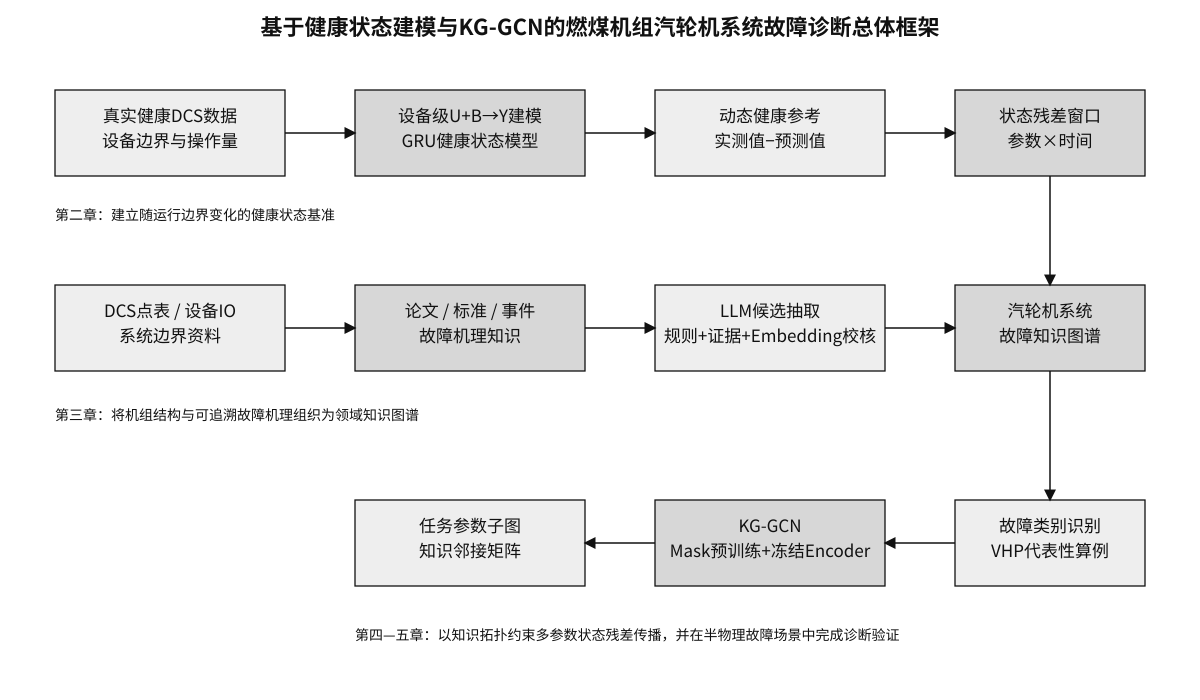
\includegraphics[width=0.98\textwidth]{figures/ch1/fig1_overall_framework.pdf}%
  \else
    \ThesisChOneOriginalFbox{#1}%
  \fi
}
\section{引言}
\label{sec:introduction}

\subsection{研究背景及意义}

在“双碳”目标与新型电力系统建设持续推进的背景下，我国电源结构正发生显著变化。国家能源局发布的2025年全国电力统计数据显示，截至2025年底，全国累计发电装机容量达到38.9亿kW，其中太阳能发电装机容量达到12.0亿kW，风电装机容量达到6.4亿kW\cite{NEA2026PowerStatistics}；国家统计局进一步指出，2025年可再生能源装机总量达到23.4亿kW，火电装机容量约15.4亿kW，占全国发电装机容量的比重首次降至40\%以下\cite{NBS2026EnergyTransition}。随着风电、光伏等波动性新能源大规模接入，电力系统对可调节电源的快速响应、深度调峰和宽负荷运行能力提出了更高要求。与此同时，煤电在我国电力安全保供和系统调节中仍承担重要的支撑作用，其功能定位正在由传统主体电源逐步向基础保障性、系统调节性电源转变。国家发展改革委、国家能源局发布的《新一代煤电升级专项行动实施方案（2025--2027年）》明确提出推进煤电向清洁低碳、安全可靠、高效调节和智能运行方向升级，并进一步强化快速变负荷、深度调峰和启停调峰能力\cite{NDRC2025CoalPowerUpgrade}。因此，在高比例新能源电力系统中，如何保证燃煤机组在频繁变工况运行条件下仍具有较高的安全性、可靠性和运行经济性，已成为煤电智能化转型过程中需要重点解决的问题。

燃煤机组灵活运行能力的提升并非单纯依赖锅炉侧调节，其本质上涉及锅炉、汽轮机及回热系统等多环节之间的动态能量协调。已有研究表明，随着可再生能源渗透率提升，传统燃煤机组需要在更低最小负荷、更高爬坡速率以及更频繁负荷循环条件下运行，机组偏离设计工况的程度显著增加\cite{GonzalezSalazar2018Flexibility}。汽轮机作为燃煤机组实现蒸汽热能向机械能转换的核心设备，是负荷调节过程中直接响应蒸汽流量与热力边界变化的关键环节。Yu等针对330~MW亚临界机组和1000~MW超超临界机组的研究指出，新能源并网背景下火电机组非设计工况运行趋于频繁，而汽轮机调节级的流量特性、效率特性及出口参数直接关系到机组灵活运行过程中的效率与安全\cite{Yu2020HybridDigitalTwin}。由此可见，汽轮机系统运行状态能否被准确表征，是燃煤机组实现宽负荷安全运行和灵活调节的重要基础。

大型燃煤机组汽轮机并非单一设备，而是由多级汽缸、再热系统、抽汽回热系统、凝汽器及其相关管路共同组成的强耦合热力系统。以二次再热汽轮机为例，主蒸汽首先进入超高压缸做功，排汽经一次再热后进入高压缸，再经二次再热进入中压缸和低压缸，并通过多级抽汽向回热系统提供热源，最终由凝汽器建立低压缸排汽边界。不同设备之间通过蒸汽流动、压力传递、能量交换以及控制调节形成显著的上下游耦合关系。Zhang等基于600~MW燃煤机组构建了汽轮机全工况模型，将汽轮机级组、再热器、抽汽管路、加热器及凝汽器等划分为多个耦合子模型，并利用实际运行数据验证了模型对不同负荷运行参数以及典型设备异常状态的表征能力\cite{Zhang2018AllCondition}。该研究说明，汽轮机系统状态并不能由单一测点或单一设备独立刻画，而应结合运行边界和设备间热力关联对系统状态进行整体分析。

% [图1占位] 燃煤机组汽轮机系统及主要运行边界示意图
% 建议内容：主蒸汽 -> VHP -> 一次再热 -> HP -> 二次再热 -> IP -> LP -> 凝汽器；
% 同时标示抽汽回热支路以及主蒸汽参数、再热蒸汽参数、机组负荷、凝汽器背压等外部运行边界。

频繁升降负荷和偏离设计工况运行还会增加汽轮机关键部件状态变化与性能退化识别的难度。一方面，负荷、主再热蒸汽参数、抽汽状态以及凝汽器背压等正常运行边界变化本身即可引起汽缸压力、温度、流量及效率参数的大幅波动，使固定阈值或设计工况基准难以直接用于长期在线评价；另一方面，快速负荷变化和频繁启停会提高关键部件的热机械载荷水平。Banaszkiewicz针对汽轮机转子开展的在线热应力监测研究表明，高灵活性运行条件下启停过程和负荷变化会导致关键部件承受显著热应力与低周疲劳载荷，因此有必要利用在线测量和数学模型持续监测关键状态\cite{Banaszkiewicz2016ThermalStress}。此外，汽轮机在长期运行过程中还可能出现叶片表面粗糙度增加、固体颗粒侵蚀、汽封磨损及叶片沉积等通流部件退化。Kubiak等通过实际汽轮机检修案例表明，这类部件退化能够通过关键压力及通流性能参数的变化在运行阶段被识别，并在后续检修中得到验证\cite{Kubiak2002TurbineDegradation}。因此，面向长期在线运行建立能够区分正常工况变化与真实设备状态偏离的监测方法，对汽轮机早期异常识别和检修决策具有重要工程意义。

传统汽轮机性能监测通常建立在热平衡、级组效率和流量特性等机理计算基础上，具有较好的物理解释性，但其在线应用精度容易受到测量不确定性、结构参数缺失以及非设计工况模型误差影响。Jiang等在燃煤机组汽轮机在线性能监测研究中指出，蒸汽循环热平衡分析高度依赖流量等关键测量的准确性，并利用数据协调方法降低测量不确定性对热耗率和性能监测结果的影响\cite{Jiang2014DataReconciliation}。与此同时，随着分布式控制系统（Distributed Control System, DCS）和厂级监控信息系统长期积累高频运行数据，利用数据驱动模型学习运行边界与设备状态之间的正常映射关系成为可能。Dettori等分别采用热力学混合模型和神经网络模型开展汽轮机在线监测建模，并利用高压汽轮机现场数据验证了模型预测能力\cite{Dettori2017MonitoringModels}；Yu等进一步将机理信息与运行数据融合用于全工况汽轮机调节级数字孪生，实现了不同运行范围内出口压力和温度等关键参数的高精度预测\cite{Yu2020HybridDigitalTwin}。这些研究表明，基于运行数据建立正常状态参考模型，可以为复杂变工况下汽轮机状态监测提供不同于固定设计基准的动态健康参照。

从故障诊断角度看，汽轮机局部异常往往不会局限于故障源所在的单一参数，而可能沿蒸汽通流、抽汽回热和压力边界关系向上下游设备传播，最终表现为多个热工参数的协同偏离。因此，仅依赖单测点阈值或将全部测点视为相互独立的特征变量，难以完整描述复杂故障的传播过程。面向燃煤机组汽轮机系统开展状态监测与故障诊断研究，一方面需要建立适应宽负荷运行条件的健康状态模型，在给定运行边界下获得关键参数的正常参考值，从而削弱正常工况迁移对异常识别的干扰；另一方面还需要充分利用汽轮机设备拓扑、介质流向及故障机理等先验知识，描述异常参数之间具有物理意义的结构关联，为后续故障类型识别和传播路径分析提供依据。由此构建从“正常状态表征—异常偏离提取—系统关联诊断”逐层递进的技术体系，不仅能够提升燃煤机组汽轮机在复杂运行条件下的状态感知能力，也可为故障早期预警、故障定位和状态检修提供数据与知识支撑，具有重要的理论研究意义和工程应用价值。

\subsection{燃煤机组汽轮机系统状态监测及故障诊断研究现状}

\subsubsection{基于机理驱动的状态监测及故障诊断方法}

基于机理驱动的状态监测及故障诊断方法以设备结构、热力过程和守恒关系为基础，通过建立能够表征健康状态的数学模型，将实际测量结果与模型计算结果进行比较，并依据效率、流量、压力、温度或残差等指标判断设备状态。汽轮机系统具有明确的质量流动和能量转换过程，因此质量守恒、能量守恒、蒸汽热力性质、级组效率以及通流能力等长期以来都是其性能评价和故障诊断的重要理论基础。与完全依赖统计相关性的方法相比，机理驱动方法能够将状态变化对应到具体热力过程或部件性能变化，其诊断结果通常具有较明确的工程物理含义。

早期汽轮机热力诊断研究主要通过建立正常参考状态并比较实际性能偏差来识别部件异常。Zaleta-Aguilar等提出面向动力系统部件的热力表征方法，利用焓变、熵变及质量流量比等参数构造参考性能状态（Reference Performance State, RPS），并在汽轮机、凝汽器、换热器和泵等对象上分析部件内部退化及外部诱发异常对参考状态的偏离\cite{Zaleta2004ThermoCharacterization}。该类方法的核心思想是先依据设计信息、热力过程与仿真计算确定无故障状态，再利用实际运行参数与健康基准之间的偏差进行状态评价。Kubiak等进一步针对叶片粗糙度、喷嘴或叶片侵蚀、汽封间隙变化和沉积等汽轮机通流部件退化开展案例研究，通过关键压力和简化流量关系识别部件性能变化，并利用停机检修结果对诊断结论进行了验证\cite{Kubiak2002TurbineDegradation}。这说明以通流能力、压力分布和级组性能变化为核心的热力参数能够较直接地反映汽轮机内部通流状态。

随着机组运行工况不断扩展，单一设计点下的性能基准难以覆盖宽负荷条件，研究重点逐渐由静态热平衡诊断向全工况动态模型与在线状态估计发展。Zhang等依据汽轮机各级组及回热系统的物理过程建立了600~MW机组全工况仿真模型，将汽轮机、再热器、抽汽管路、给水加热器和凝汽器等多个模块耦合起来，实现不同运行负荷下系统参数的动态计算\cite{Zhang2018AllCondition}。Yu等则围绕汽轮机调节级构建机理与数据融合的数字孪生模型，根据阀门流量关系和级组热力特性计算调节级状态，并通过运行数据辨识和修正模型参数，使模型能够用于不同工况下出口压力、温度等性能参数的在线监测\cite{Yu2020HybridDigitalTwin}。对于实际机组测量误差问题，Jiang等将非线性数据协调引入汽轮机在线性能监测，在质量与能量平衡等约束下对运行测量数据进行校正，以提高热耗率及相关性能参数计算的可信度\cite{Jiang2014DataReconciliation}。上述工作表明，利用机理约束建立随运行边界变化而变化的正常状态模型，是提高宽工况汽轮机性能监测准确性的有效途径。

除直接计算热力性能指标外，基于状态观测器和残差分析的模型诊断方法也被用于锅炉—汽轮机耦合系统。Madrigal-Espinosa等基于实际电厂低、中、高负荷数据建立准线性参数时变（quasi-linear parameter varying, quasi-LPV）锅炉—汽轮机模型，并设计Luenberger型观测器产生模型残差，通过自适应阈值完成关键传感器故障检测与隔离\cite{Madrigal2017BoilerTurbineFDI}。该研究说明，模型预测与实际观测之间的残差不仅可以反映系统状态偏离，还可以通过自适应基准减少负荷变化造成的误报警。Banaszkiewicz则从热机械安全角度利用实时温度和机理模型在线估计汽轮机转子热应力，为启停及变负荷过程中的寿命消耗监测和运行控制提供依据\cite{Banaszkiewicz2016ThermalStress}。因此，机理模型既可以直接形成性能指标，也可以作为生成健康参考值和状态残差的基础。

总体而言，机理驱动方法能够充分利用汽轮机质量守恒、能量守恒和通流特性等先验规律，在故障机理解释、状态参数推演和诊断结果可信度方面具有明显优势。然而，大型汽轮机系统包含多级汽缸、再热器、抽汽回热设备及凝汽器等多个耦合部件，精细模型往往需要较完整的设备结构、设计工况、阀门特性、级组参数和蒸汽物性信息；实际运行中的测量误差、设备老化、检修改造及长期性能漂移又会造成模型参数与真实对象逐渐偏离。虽然数据协调、参数辨识及混合建模能够缓解上述问题\cite{Jiang2014DataReconciliation,Yu2020HybridDigitalTwin}，但对于需要长期在线部署的大规模机组而言，逐设备建立并持续修正高精度机理模型仍具有较高的专业知识和维护成本。因此，在保留必要物理边界和设备拓扑信息的同时，利用长期运行数据自主学习复杂非线性状态关系，成为汽轮机状态监测与故障诊断的重要研究方向。

\subsubsection{基于数据驱动的状态监测及故障诊断方法}

随着DCS、汽轮机监视仪表系统（Turbine Supervisory Instrumentation, TSI）及厂级信息系统的持续建设，燃煤机组积累了大量包含负荷、压力、温度、流量、阀位以及设备状态信息的历史运行数据。基于数据驱动的方法无需完整求解汽轮机内部复杂热力过程，而是利用历史样本建立输入运行条件与目标状态参数之间的统计或非线性映射，或者直接学习健康数据在高维特征空间中的正常分布。按照模型任务不同，相关研究主要可以分为正常状态建模与参数预测、无监督异常检测以及有监督故障分类等方向。

正常状态建模的基本思想是在健康运行数据上学习设备随工况变化的正常响应关系，以动态参考值替代固定设计值。Cao等针对凝汽式汽轮机末级组湿蒸汽区排汽焓难以准确获取的问题，分析影响末级组相对内效率的运行因素，并采用组合BP神经网络建立正常相对内效率计算模型，其宽工况测试结果与理论计算结果具有较好一致性，为末级组状态监测提供了数据驱动正常值基准\cite{Cao2016LastStageNormalValue}。Dettori等比较了热力学混合模型和神经网络模型在汽轮机在线监测中的应用，利用高压汽轮机现场运行数据预测关键状态参数，说明神经网络可以在缺少部分直接测量量时学习复杂设备的正常运行映射\cite{Dettori2017MonitoringModels}。这些工作表明，将运行工况作为模型条件并预测设备正常状态，是削弱非设计工况影响的一种可行思路。

汽轮机运行数据具有明显的时间相关性，频繁升降负荷时当前状态不仅与瞬时输入有关，还受到前序运行过程和热惯性的影响。因此，循环神经网络等时序模型逐渐被用于汽轮机动态状态监测。Li等针对传统稳态评价方法在动态运行过程中的适应性不足问题，将机理分析与数据特征选择相结合，并利用长短期记忆网络（Long Short-Term Memory, LSTM）建立级组性能退化预警模型；实验结果显示，考虑时间序列信息有助于提升动态工况下性能退化识别能力\cite{Li2021LSTMStageWarning}。近年来，针对多工况状态迁移问题，Chen等构建了基于多高斯过程自适应迁移学习的汽轮机在线无监督状态监测框架，将环境变化、功率需求变化及人工调整引起的不同运行模式显式纳入监测过程，并通过两级判据区分正常模式迁移与异常状态；该方法在实际汽轮机数据上完成验证，且无需故障标签\cite{Chen2023AdaptiveTransfer}。这类研究说明，宽工况状态监测的关键不仅是提高单一工况下的预测精度，还需要避免将正常工况迁移错误判断为设备异常。

考虑到电站重大设备故障发生频率低且出现异常后通常会及时停机或处置，真实汽轮机故障样本往往远少于正常样本，无监督或仅依赖健康数据的异常检测方法受到广泛关注。Ko等采用集成降噪自编码器建立汽轮机正常状态模型，并根据模型输出与残差联合分布构造动态阈值，以降低正常状态波动造成的误报警，同时利用残差敏感度识别与异常相关的监测信号\cite{Ko2022DynamicThresholdAE}。Zhai等利用真实660~MW机组运行数据构建基于卷积自编码器的汽轮机故障预警模型，通过模型预测输出与实际运行数据之间的偏差识别异常，并结合混合信息增益筛选多维传感器特征\cite{Zhai2024CAEWarning}。Xu和Zhang进一步采用增强LSTM变分自编码器对高维汽轮机时序数据进行无监督表示学习，将潜变量和重构误差融合为异常特征，并在实际工业汽轮机数据上进行验证\cite{Xu2025LSTMVAE}。从这些研究可以看出，基于正常数据学习健康行为并利用预测或重构偏差表征异常，能够在缺少完整故障标签的情况下充分利用电厂长期积累的健康运行样本。

在明确故障类型的诊断任务中，支持向量机、神经网络、模糊推理及其组合模型也被广泛应用。Salahshoor等面向工业汽轮机构建SVM与自适应神经模糊推理系统（Adaptive Neuro-Fuzzy Inference System, ANFIS）融合的故障检测与诊断方法，通过有序加权平均实现多分类器信息融合，并在包含高压、中压和低压部分的工业汽轮机仿真对象上验证了多类早期故障识别能力\cite{Salahshoor2010SVMANFIS}。此类监督分类方法能够直接建立多变量运行特征与故障类别之间的映射，在训练故障模式与实际测试模式一致时通常具有较高分类效率，但其性能较大程度取决于故障样本覆盖范围、类别均衡程度以及训练和实际运行工况之间的数据分布一致性。

传统神经网络和机器学习模型通常将多测点数据组织为规则向量或矩阵进行特征学习，而汽轮机的汽缸、再热器、抽汽系统和凝汽器之间具有明确的物理连接关系，故障影响也可能沿蒸汽流动和设备连接关系逐级传播。为显式利用复杂系统中的结构信息，近年来图神经网络（Graph Neural Network, GNN）逐渐被引入工业故障诊断。Zhang和Hu针对汽轮机系统首先依据系统机理建立过程图，并进一步构建包含潜在故障节点和传播关系的故障图，采用GNN学习故障节点表示并通过链路预测推断汽轮机泄漏故障传播路径，验证了以图结构表达汽轮机设备关系和故障传播的可行性\cite{ZhangHu2021FaultPropagationGNN}。在通用工业过程领域，Jia等根据工艺流程图建立变量拓扑图，将自注意力、图卷积和图池化结合用于故障诊断，使模型特征传播过程受到实际流程拓扑约束\cite{Jia2023TopologyGuidedGraph}；Han等则将过程知识模型与GNN结合，通过知识约束减少因纯数据因果发现产生的冗余连接，并用于复杂工业过程的故障根因分析\cite{Han2022KnowledgeEnhancedGNN}。这些研究表明，将设备拓扑、工艺流程及领域知识转化为图结构，可以使数据驱动模型在提取统计特征之外进一步利用具有物理意义的参数关联关系，为复杂热力系统的故障传播建模和诊断解释提供新的技术路径。

综上，数据驱动方法在非线性拟合、时序特征学习和复杂高维数据处理方面具有明显优势，并已经从传统监督分类逐渐发展到健康状态建模、无监督异常检测和知识增强图学习等多种技术路线。然而，面向燃煤机组汽轮机系统的长期在线应用仍存在若干不足：一是汽轮机参数随负荷和热力边界显著变化，若直接使用原始参数进行异常检测或故障分类，正常工况迁移与真实故障造成的状态偏离可能产生特征混叠\cite{Li2021LSTMStageWarning,Chen2023AdaptiveTransfer}；二是高质量故障样本获取困难，仅依赖监督学习难以充分利用长期积累的大量健康运行数据\cite{Ko2022DynamicThresholdAE,Chen2023AdaptiveTransfer}；三是多数基于规则向量的数据驱动模型未显式表达汽轮机设备之间的蒸汽流动、能量传递和故障传播关系，而现有图学习研究虽然证明了拓扑知识在工业故障诊断中的价值\cite{ZhangHu2021FaultPropagationGNN,Jia2023TopologyGuidedGraph,Han2022KnowledgeEnhancedGNN}，但如何将汽轮机健康状态模型得到的动态异常信息与系统级领域知识进行统一融合，仍具有进一步研究和工程应用价值。

\subsection{现有研究与应用存在的问题}

根据上述研究现状，现有燃煤机组汽轮机状态监测及故障诊断方法已在热力性能计算、正常行为建模、异常检测及智能分类等方面取得较多成果，但在复杂变工况和系统级故障诊断场景下仍存在以下问题。

（1）\textbf{正常工况变化与设备异常在原始参数空间中存在混叠。} 汽轮机压力、温度、流量及抽汽状态不仅受设备健康程度影响，还随负荷、主再热蒸汽参数、凝汽器背压及运行策略改变而发生显著变化。已有研究已经从动态性能建模和多运行模式监测角度指出，传统稳态或单模式模型在频繁负荷变化条件下容易降低监测灵敏度，正常模式切换也可能造成误报警\cite{Li2021LSTMStageWarning,Chen2023AdaptiveTransfer}。因此，仅依据实际测量值的绝对变化识别故障难以稳定适用于宽负荷运行场景，需要首先建立能够表征给定运行边界下健康响应的正常状态模型，并利用实际状态相对健康参考的偏离量提取异常特征。

（2）\textbf{纯数据驱动诊断模型难以显式利用汽轮机系统的物理拓扑和故障传播知识。} 大型汽轮机由超高压缸、高压缸、中压缸、低压缸、再热系统、抽汽回热系统和凝汽器等多个设备构成，参数之间通过蒸汽流动、压力传递和能量交换形成明确结构关系。当局部故障发生时，异常特征可能沿设备连接逐层传播。现有向量化机器学习模型主要依赖样本中的统计相关性，其内部特征交互不必然与真实热力拓扑一致。汽轮机故障传播GNN及流程拓扑引导图学习研究已经证明，显式引入系统结构能够为故障特征聚合和传播路径推断提供有效约束\cite{ZhangHu2021FaultPropagationGNN,Jia2023TopologyGuidedGraph}。因此，有必要进一步将汽轮机设备、参数、异常现象和故障机理等运行知识结构化表达，并作为诊断模型的拓扑先验。

（3）\textbf{真实高质量故障样本稀缺，监督式诊断模型训练受到限制。} 汽轮机属于高可靠性重大旋转设备，异常状态通常会被及时处置，重大故障发生频率较低，导致现场长期数据中健康样本数量远高于有效故障样本。Ko等和Chen等均指出，汽轮机真实故障数据难以充分获取，因而采用仅依赖正常数据或不依赖故障标签的无监督监测策略\cite{Ko2022DynamicThresholdAE,Chen2023AdaptiveTransfer}。若直接利用少量有标签故障样本从零开始训练高容量深度分类模型，容易受到样本数量和类别分布影响。因此，需要在故障分类之前充分利用大量无标签健康运行数据学习汽轮机参数之间的正常关联结构，再利用有限故障样本完成判别边界训练。

（4）\textbf{健康状态监测与系统级故障诊断之间缺少统一的信息衔接。} 现有研究中，一类方法侧重于建立正常行为模型并依据预测误差或重构误差检测异常\cite{Dettori2017MonitoringModels,Ko2022DynamicThresholdAE,Zhai2024CAEWarning}，另一类方法则直接基于故障样本建立分类器或利用图结构推断故障关系\cite{Salahshoor2010SVMANFIS,ZhangHu2021FaultPropagationGNN}。两类研究分别解决“运行状态是否偏离健康状态”和“异常属于何种故障或如何传播”的问题，但在实际汽轮机系统中二者具有天然的前后联系。若能够将健康状态模型生成的参数偏差作为动态故障表征，并进一步在汽轮机知识拓扑中进行关联特征聚合，即可形成从正常状态基准、异常特征提取到故障类别识别的连续诊断链路。

基于上述问题，本文面向燃煤机组汽轮机系统构建“健康状态建模—动态残差表征—知识图谱约束—图卷积故障诊断”的统一技术框架。首先利用正常运行数据建立适应运行边界变化的设备级健康模型，将实际测量值与健康模型预测值之间的偏差作为状态异常表征；随后利用运行生产资料建立汽轮机故障知识图谱，将设备拓扑和参数关联关系转化为图卷积网络可计算的邻接结构；最后在图拓扑约束下聚合多参数动态残差，实现故障类别识别及关联特征分析。

\subsection{论文主要研究内容}

本文以某燃煤机组汽轮机系统为研究对象，围绕复杂变工况下正常状态表征不足、系统拓扑知识利用不充分及故障样本有限等问题，研究基于健康状态模型与知识图谱图卷积网络的汽轮机故障诊断方法。全文总体技术路线如图~\ref{fig:overall_framework}所示，主要研究内容如下。

（1）\textbf{构建基于GRU的燃煤机组汽轮机系统健康状态监测方法。} 根据汽轮机热力系统的介质流动关系和设备边界，将运行操作变量与上游/外部热力边界作为模型输入，以反映设备正常状态的关键压力、温度等参数作为模型输出，建立设备级健康状态预测模型。考虑汽轮机运行参数具有动态迟延和时间相关特性，引入门控循环单元（Gated Recurrent Unit, GRU）学习历史时间窗口内的多变量动态映射，并设置ANN、TCN及iTransformer等模型进行对比。以超高压缸为典型对象开展工程算例，通过实际运行数据验证健康模型对复杂运行边界下正常参数变化的表征能力，并进一步由实际观测值与模型预测值构造标准化动态残差，为后续故障诊断提供状态特征。

（2）\textbf{构建面向汽轮机系统故障诊断的运行知识图谱。} 面向汽轮机本体及相关热力系统，综合设备说明、运行规程、系统拓扑、故障案例及相关运行生产资料，对设备、监测参数、异常现象、故障类型和处置等知识实体进行统一定义；通过文本知识抽取、关系校验和实体标准化等过程形成结构化三元组，建立覆盖超高压缸、高压缸、中压缸、低压缸、再热及抽汽回热等关键环节的汽轮机故障知识图谱。进一步从知识图谱中提取与状态监测参数对应的关联关系，构建可用于图卷积计算的参数邻接矩阵。

（3）\textbf{提出融合健康状态残差与知识图谱的KG-GCN故障诊断方法。} 将健康模型产生的连续标准化残差按照滑动时间窗口映射为知识图谱中参数节点的动态特征，并以知识图谱得到的参数邻接矩阵作为图卷积网络的结构输入，使不同参数的异常信息沿具有实际工程意义的关联路径进行特征传播与聚合。针对故障标签有限的问题，首先利用大量无标签运行残差窗口对图卷积编码器进行掩码重构预训练，使模型学习汽轮机参数在知识拓扑约束下的关联特征，再利用有限有标签故障样本训练故障分类层，实现汽轮机系统故障识别。

（4）\textbf{开展典型对象故障诊断实验并验证方法有效性。} 以超高压缸及其关联热力参数为典型对象构建故障诊断算例，采用准确率、精确率、召回率及Macro-F1等指标评价诊断性能，并与传统数据驱动诊断模型进行对比。同时通过去除健康残差表征或知识拓扑约束等消融实验，分别分析健康状态建模与知识图谱对故障诊断性能的贡献，并结合异常参数及图节点关联关系分析典型故障的特征传播过程。

\begin{figure}[htbp]
    \centering
    % \includegraphics[width=0.96\textwidth]{figures/overall_framework.pdf}
    \fbox{\parbox[c][5.0cm][c]{0.92\textwidth}{\centering
    图占位：基于健康状态建模与KG-GCN的燃煤机组汽轮机系统故障诊断总体框架\\[0.5em]
    DCS健康运行数据 $\rightarrow$ GRU健康模型 $\rightarrow$ 标准化动态残差\\
    运行规程/说明书/故障资料 $\rightarrow$ 知识抽取 $\rightarrow$ 汽轮机故障知识图谱\\
    动态残差窗口 + 参数邻接矩阵 $\rightarrow$ KG-GCN $\rightarrow$ 故障类别与关联特征分析}}
    \caption{基于健康状态建模与KG-GCN的燃煤机组汽轮机系统故障诊断总体框架}
    \label{fig:overall_framework}
\end{figure}

\endgroup

% Final Chapter 2 wrapper. Historical figure placeholders are materialized by scripts/apply_final_figures.py in the isolated build copy.
\begingroup
\setlength{\tabcolsep}{2.5pt}
\let\ThesisChTwoOriginalSubsubsection\subsubsection
\renewcommand{\subsubsection}[1]{%
  \ifstrequal{#1}{数据集及实验设置}{%
    \par\noindent\textit{评价口径说明：}最终24个状态点由后续故障诊断的统一参数节点映射规则确定，不依据ANN、TCN、iTransformer-small或GRU在独立测试集上的预测精度进行筛选。网络训练阶段仍保留27个候选输出，CT132A、CT151A和CT152A仅不纳入本文统一的24点评价与诊断映射口径。\par
  }{}%
  \ThesisChTwoOriginalSubsubsection{#1}%
}
% ==========================================================================
% 第二章  燃煤机组汽轮机系统状态监测建模方法（v4）
% 对齐杨昊东式章节功能与真实VHP工程数据；本文件为Ch2审计事实源。
% ==========================================================================

\section{燃煤机组汽轮机系统状态监测建模方法}
\label{sec:gru_monitoring_v4}

\subsection{引言}

燃煤机组汽轮机系统在宽负荷、频繁变工况条件下运行时，设备压力、温度和流量等状态参数不仅受到设备健康状态影响，还会随入口蒸汽边界、负荷水平及操作调节持续变化。若直接将某一设计值或固定历史均值作为正常状态基准，容易把正常工况迁移误判为设备异常。因此，建立能够随运行边界动态变化的健康状态参考，是后续利用状态偏差信息开展故障诊断的基础。

本文按照汽轮机实际热力过程将系统划分为VHP、一次再热、HP、二次再热、IP、LP及凝汽器等设备级建模对象，并统一采用“操作变量$U$+热力边界$B\rightarrow$设备状态$Y$”的建模方式。模型输入仅使用当前设备能够直接获得的真实DCS操作量和边界量，不将上游模型预测输出继续串联为下游模型输入，从而避免多设备串联预测造成误差累积。考虑汽轮机过程参数存在明显的时间迟延与历史依赖，本章采用门控循环单元（Gated Recurrent Unit，GRU）建立设备级健康状态预测模型，并以VHP作为代表性对象开展完整工程算例。

本章首先说明汽轮机系统设备级建模对象及其输入输出边界；随后给出GRU动态建模方法及训练策略；在此基础上构建VHP健康状态模型，并通过2024年5月正常运行数据训练、2024年6月独立测试，与ANN、TCN和iTransformer-small进行对比，最后分析不同状态参数的可建模性及模型适用边界。

\subsection{汽轮机系统设备级状态监测建模对象}
\label{subsec:turbine_device_objects_v4}

汽轮机热力系统主通流可概括为“主蒸汽--VHP--一次再热--HP--二次再热--IP--LP--凝汽器”。各设备之间通过蒸汽介质持续传递热力状态，同时还与抽汽回热、给水和冷端系统形成耦合。为了使设备健康模型具有明确物理边界，本文不采用整机统一黑箱输入输出，而是依据介质流向和实际DCS测点对系统进行设备级划分。

设第$m$个设备在时刻$t$的操作变量、热力边界和状态输出分别为$\mathbf U_m(t)$、$\mathbf B_m(t)$和$\mathbf Y_m(t)$，则设备健康状态映射可表示为
\begin{equation}
\hat{\mathbf Y}_m(t)=f_m\left(\mathbf U_m(t-L+1:t),\mathbf B_m(t-L+1:t);\theta_m\right),
\end{equation}
式中：$L$为历史时间窗口长度；$\theta_m$为模型参数；$\hat{\mathbf Y}_m(t)$为给定当前操作和边界条件下的设备健康状态预测值。模型仅用于学习健康运行数据中的条件响应关系，不在本章直接承担故障分类任务。

设备边界的确定遵循三个原则：一是输入量应位于设备上游或外部边界，避免使用本级近出口量作为输入形成信息泄漏；二是输出量应能够反映设备本体及直接热力接口状态；三是所有输入输出均对应实际可获取DCS测点。对于相邻设备，上一设备的真实DCS出口测量量可以作为下一设备的实际入口边界，但不使用上一模型的预测值进行级联。

依据上述原则，本文当前构建的汽轮机系统状态监测对象包括VHP、RH1、HP、RH2、IP、LP和两个凝汽器等，主要对象及边界见表~\ref{tab:system_objects_v4}。

\begin{table}[htbp]
    \centering
    \caption{汽轮机系统主要设备级状态监测对象}
    \label{tab:system_objects_v4}
    \begin{tabular}{p{1.3cm}p{2.6cm}p{4.4cm}p{4.4cm}p{1.5cm}}
        \toprule
        编号 & 对象 & 主要输入边界 & 主要状态输出 & 数据可用性 \\
        \midrule
        M1 & VHP & 主蒸汽P/T、阀位、负荷、主汽流量 & VHP本体、一级抽汽、冷再接口及缸体热状态 & 完整 \\
        M2 & RH1 & VHP/冷再入口、再热调节相关边界 & 一次高温再热出口P/T及相关状态 & 可建模 \\
        M3 & HP & 一次高温再热入口P/T及工况边界 & HP本体及后续热力接口状态 & 完整 \\
        M4 & RH2 & HP排汽及二次再热入口边界 & 二次高温再热出口P/T及相关状态 & 可建模 \\
        M5 & IP & 二次高温再热入口及工况边界 & IP本体及抽汽相关状态 & 可建模 \\
        M6 & LP & IP/连通管相关入口及冷端边界 & LP本体及低压抽汽状态 & 可建模 \\
        M7/M8 & CND1/2 & LP排汽、循环水及冷端边界 & 真空、凝结水和冷端相关状态 & 可建模 \\
        \bottomrule
    \end{tabular}
\end{table}

上述设备划分用于统一全文“设备级健康状态建模”的物理接口。考虑本研究当前已完成并具有完整独立测试结果的对象为VHP，后续算法对比与状态监测结果分析均以VHP为代表性算例，其余设备用于说明该方法可按相同边界规则扩展，而不在本章宣称已经完成同等独立实验验证。

\subsection{GRU动态健康状态建模方法}
\label{subsec:gru_method_v4}

\subsubsection{GRU基本结构}

循环神经网络能够通过隐藏状态在相邻时间步之间传递历史信息，但传统RNN在较长时间序列训练中容易出现梯度消失或梯度爆炸。GRU通过更新门和重置门控制历史信息保留与当前输入写入，在较少参数规模下能够学习工业过程中的短期动态和一定历史记忆\cite{Cho2014GRU}。

对于时刻$t$的输入向量$\mathbf x_t$和上一时刻隐藏状态$\mathbf h_{t-1}$，GRU更新门$\mathbf z_t$和重置门$\mathbf r_t$分别定义为
\begin{equation}
\mathbf z_t=\sigma(W_z\mathbf x_t+U_z\mathbf h_{t-1}+\mathbf b_z),
\end{equation}
\begin{equation}
\mathbf r_t=\sigma(W_r\mathbf x_t+U_r\mathbf h_{t-1}+\mathbf b_r),
\end{equation}
式中：$\sigma(\cdot)$为Sigmoid激活函数；$W_z$、$U_z$、$W_r$、$U_r$为可学习权重；$\mathbf b_z$和$\mathbf b_r$为偏置项。更新门决定上一时刻隐藏状态有多少被保留，重置门控制历史信息在候选状态计算中的参与程度。

候选隐藏状态为
\begin{equation}
\tilde{\mathbf h}_t=\tanh\left(W_h\mathbf x_t+U_h(\mathbf r_t\odot\mathbf h_{t-1})+\mathbf b_h\right),
\end{equation}
最终隐藏状态更新为
\begin{equation}
\mathbf h_t=(1-\mathbf z_t)\odot\mathbf h_{t-1}+\mathbf z_t\odot\tilde{\mathbf h}_t,
\end{equation}
式中$\odot$表示逐元素乘法。通过门控机制，GRU能够在负荷变化、阀位调节以及蒸汽热力边界变化过程中保留对当前状态预测有价值的历史信息。

本文采用固定长度历史窗口构造设备输入序列。对于VHP，窗口长度为24个采样点，即24 min。设单时刻输入维数为$p$，则一个样本的输入矩阵为
\begin{equation}
X_t=[\mathbf x_{t-L+1},\ldots,\mathbf x_t]^{\mathrm T}\in\mathbb R^{L\times p}.
\end{equation}
GRU对整个窗口进行编码，取末时刻隐藏状态作为当前时刻的动态特征，并通过线性层同步预测$q$个设备状态量。

\subsubsection{多输出回归与损失函数}

汽轮机设备状态量同时包含压力、温度等不同物理量，原始量纲和数值范围差异较大。为避免大数值量纲在损失中占据主导，训练阶段首先使用训练集统计量对输入和输出分别进行标准化。对于第$j$个输出变量，标准化形式为
\begin{equation}
y_j^{*}=\frac{y_j-\mu_j}{s_j},
\end{equation}
式中$\mu_j$和$s_j$分别为训练集第$j$个变量的均值与标准差。验证集和测试集均只使用训练集得到的$\mu_j$和$s_j$，避免未来数据参与统计量估计。

模型采用标准化空间中的平均均方误差作为训练目标：
\begin{equation}
\mathcal{L}_{\mathrm{MSE}}=\frac{1}{N_bq}\sum_{i=1}^{N_b}\sum_{j=1}^{q}\left(y_{ij}^{*}-\hat{y}_{ij}^{*}\right)^2,
\end{equation}
其中$N_b$为批样本数，$q$为输出维度。标准化后，各输出维度在训练阶段具有相近数值尺度，使多输出任务能够在统一损失中共同参与优化。

在GRU输出后，本文引入LayerNorm对单样本隐藏特征进行归一化。LayerNorm根据同一层神经元特征计算均值和方差，其训练与测试阶段计算方式一致，并适用于循环网络隐藏状态稳定化\cite{Ba2016LayerNorm}。随后采用Dropout(0.05)进行轻度正则化，在训练过程中随机抑制部分隐藏特征，降低特征之间过度共适应的风险\cite{Srivastava2014Dropout}。由于本文网络规模较小，Dropout率设置较低，目的在于保持主要动态信息的同时提供必要正则化，而非通过较强随机失活改变网络表达能力。

\subsubsection{BPTT与参数优化}

GRU训练过程采用时间反向传播（BPTT）。在前向阶段，同一组GRU参数在$L$个时间步上重复使用，输入序列依次更新隐藏状态并形成多输出预测；计算回归损失后，梯度从输出层返回隐藏状态，并沿时间展开结构反向累积至各时间步共享参数，实现历史信息路径和当前输入路径的联合优化。

本文采用AdamW优化器进行参数更新。AdamW将权重衰减与自适应梯度更新过程解耦，可在使用Adam类自适应学习率的同时保持独立的权重衰减机制\cite{Loshchilov2019AdamW}。此外，训练中采用梯度范数裁剪限制异常梯度放大，并利用ReduceLROnPlateau在验证损失长期不改善时降低学习率，使模型在训练后期以更小步长搜索稳定参数区域。上述训练策略均服务于小型设备级网络的稳定优化，不作为本文独立算法创新点。

\subsection{基于GRU的汽轮机设备级状态监测模型构建}
\label{subsec:device_model_construction_v4}

在明确汽轮机设备边界及GRU动态建模原理后，本节进一步给出面向系统级应用的统一模型构建方法。该方法的重点不在于为不同设备设计完全不同网络，而在于依据真实热力流程确定各设备的边界输入和状态输出，并以一致的数据处理和训练协议建立可比较的健康状态参考。

\subsubsection{设备级输入输出定义}

对于任一设备模型，输入序列可统一写为
\begin{equation}
\mathbf x_t=[\mathbf U_t,\mathbf B_t],
\end{equation}
其中$\mathbf U_t$表示负荷、阀位、调节量等操作变量，$\mathbf B_t$表示设备入口蒸汽状态及必要的外部边界。输出向量$\mathbf y_t$由设备本体状态及直接热力接口状态组成。对于相邻设备，上一设备真实DCS出口测点可以进入下一设备的$\mathbf B_t$，但上一模型预测值不参与下一模型输入。

该结构的作用在于把正常工况变化解释为“给定$U+B$条件下$Y$应达到的健康响应”。后续若实际$Y$与健康预测$\hat Y$发生持续偏离，则偏差信息可进一步用于构造故障诊断节点的动态特征，而无需在状态监测阶段直接设定故障阈值。

\subsubsection{数据处理与样本构造}

设备原始DCS数据首先进行有效值筛选，并剔除计划停机、检修和明确无有效采集的时间区间。对正常运行数据按自然时间顺序构造长度为$L$的连续滑动窗口，窗口内部不允许跨越停机、无效数据或大时间断点。

输入和输出标准化参数仅由训练数据计算。对于VHP月度独立测试实验，2024年5月数据用于模型训练及内部验证，2024年6月数据作为完全独立测试集，不参与网络权重更新、标准化参数估计和模型选择。通过这种划分方式，测试结果反映模型从一个月份推广至下一独立月份的状态参考能力。

\subsubsection{网络结构与训练协议}

本文设备级GRU统一采用单层GRU编码历史窗口，隐藏维度为32，随后依次连接LayerNorm、Dropout和线性输出层。以VHP为例，实际训练网络为
\begin{equation}
24\times16\rightarrow \mathrm{GRU}(32)\rightarrow \mathrm{LayerNorm}\rightarrow \mathrm{Dropout}(0.05)\rightarrow \mathrm{Linear}(27),
\end{equation}
可训练参数总数为5755。这里Linear(27)对应训练阶段27个候选状态输出；完成状态点筛选后，后续统计分析和故障诊断映射统一使用24个状态点，因此不能将实际训练网络改写为Linear(24)。

优化器采用AdamW，初始学习率为$1\times10^{-3}$，权重衰减为$1\times10^{-4}$，批量大小为4096，并使用ReduceLROnPlateau调节学习率、梯度范数裁剪5.0和验证集早停。最大训练轮数设置为300轮，模型选择仅依据训练月份内部验证集性能，不使用独立测试月份进行调参。

\subsection{VHP状态监测算例}
\label{subsec:vhp_case_v4}

\subsubsection{研究对象及输入输出配置}

VHP位于主蒸汽进入汽轮机后的首个主要膨胀设备，其入口由A/B侧主蒸汽参数和调节阀状态共同决定，排汽进入一次低温再热系统，同时设置一级抽汽支路向1号高压加热器供汽。因此，VHP既具有明确的主通流边界，又同时包含汽缸本体、抽汽支路及再热接口等多类可观测状态，适合作为设备级健康建模的代表性算例。

实际模型采用16个输入变量。主蒸汽边界包含A/B侧共12个压力和温度测点；操作与工况变量包括2个VHP调节阀实际位置、有功负荷和主蒸汽流量。输入中不加入汽轮机转速，因为正常并网运行阶段转速基本恒定；凝汽器背压属于下游冷端状态，不作为VHP直接输入；高旁状态也不作为本模型输入，只在必要时用于运行工况筛选。

训练阶段设置27个候选状态输出，最终评价与故障诊断使用24点。24点覆盖四类状态区域：VHP本体及主排汽状态、一级抽汽及1号高压加热器入口状态、VHP至一次再热接口状态，以及缸体/内部蒸汽慢变热状态。这样的输出设计使健康模型不仅描述汽缸局部压力温度，还覆盖与后续故障传播相关的直接热力接口。

\subsubsection{数据集及实验设置}

VHP健康状态模型采用2024年5月正常运行数据训练，并以2024年6月数据进行独立测试，采样周期为1 min。经有效值和连续时间窗口筛选后，训练月份可用样本数为43911，独立测试月份可用样本数为42710。为了比较不同动态建模方式，设置ANN、TCN、iTransformer-small和GRU-RNN四种模型，所有模型使用相同的输入输出变量、训练月份和独立测试月份。

ANN采用单时刻输入作为静态基线，不具有显式历史窗口。对于GRU、TCN和iTransformer-small，连续24个采样点构成一个时序输入窗口。仅保留窗口内部相邻时间戳连续的样本，完成序列构造后，GRU训练集包含43759个序列样本，独立测试集包含42595个序列样本。模型输入和输出均采用StandardScaler标准化，所有均值和标准差仅根据训练数据确定。

GRU隐藏维度为32，Dropout率为0.05，训练采用AdamW优化器，初始学习率为$1\times10^{-3}$，权重衰减为$1\times10^{-4}$，batch size为4096，并将梯度范数裁剪至5.0。模型选择阶段根据验证损失使用ReduceLROnPlateau调整学习率，确定最佳训练轮次后，在完整训练月份重新训练最终模型。上述设置用于形成本文稳定基线，不将其声称为经过全局超参数搜索得到的唯一最优组合。

模型采用$R^2$、RMSE和MAE评价单点预测性能：
\begin{equation}
R^2=1-\frac{\sum_{i=1}^{n}(y_i-\hat y_i)^2}{\sum_{i=1}^{n}(y_i-\bar y)^2},
\end{equation}
\begin{equation}
\mathrm{RMSE}=\sqrt{\frac{1}{n}\sum_{i=1}^{n}(y_i-\hat y_i)^2},\qquad
\mathrm{MAE}=\frac{1}{n}\sum_{i=1}^{n}|y_i-\hat y_i|.
\end{equation}
由于24个状态同时包含压力和温度等不同物理量，RMSE和MAE仅用于逐测点或相同量纲参数比较；跨状态总体性能采用无量纲的24点宏平均$R^2$评价。

\subsubsection{模型训练过程}

模型选择阶段训练损失和验证损失随训练轮次整体下降，并在后期进入稳定区间。最低验证MSE为0.057533，出现在epoch 161，对应训练MSE为0.043519。根据该结果，将161轮确定为最终训练轮次；随后利用完整2024年5月训练数据重新训练模型，第161轮完整训练集MSE为0.039283。图2-5同时给出训练和验证损失，并标记最佳验证轮次，以避免仅凭单一训练损失判断模型是否收敛。

训练损失仅反映模型对训练数据的拟合程度，不能单独作为状态监测模型有效性的依据。因此，本文进一步使用完全独立的2024年6月数据评价跨月份泛化性能，重点检验模型在新的运行时间区间和负荷分布下能否继续给出稳定的正常状态参考。

\subsubsection{总体状态监测性能}

在最终24个状态参数上，ANN、TCN、iTransformer-small和GRU-RNN的测试宏平均$R^2$分别为0.9087、0.9397、0.9356和0.9511。GRU取得最高总体精度，相比ANN提高0.0424，相比TCN和iTransformer-small分别提高0.0114和0.0155。需要指出，ANN作为静态基线不具有与三种时序模型相同的历史信息，因此GRU相对ANN的提升同时包含“引入时间历史”和“采用门控时序结构”两方面影响；GRU与TCN、iTransformer-small之间的比较更能反映不同动态特征提取机制的差异。

从状态分组看，GRU在VHP本体及主排汽状态Y1、一级抽汽接口Y2和VHP至RH1接口Y3上的平均$R^2$分别为0.9581、0.9634和0.9569，在缸体与内部蒸汽状态Y4上的平均$R^2$为0.8892。前三组主要由压力、主流蒸汽温度及抽汽/冷再接口状态构成，与入口边界和配汽状态之间具有较直接动态关系；Y4包含金属壁温等慢变状态，受蓄热和更长历史工况影响，其预测难度明显更高。这一分组差异与前述汽轮机参数快慢动态特性分析相一致。

逐测点统计中，GRU在24个状态点中的17个点取得四种模型最高$R^2$，其余7个点由iTransformer-small取得最优结果。由于其中部分压力点各模型本身已达到接近0.998的高精度，单纯统计“最优点数量”并不足以评价模型优劣，因此本文进一步选取具有不同动态特性的代表性状态分析预测曲线。

\subsubsection{典型状态参数预测结果}

对于超高压缸叶片级压力\#1，GRU完整测试月$R^2$达到0.9979，说明主蒸汽边界、阀门状态及负荷信息能够较充分描述该压力状态变化。压力是通流系统中响应较快的状态量，其与入口流量和级组压力分布之间关系相对稳定，因此四种模型在此类测点上通常均能获得较高精度。

对于具有更明显热惯性的排汽蒸汽温度，模型差异更加突出。超高压排汽蒸汽温度\#1上，ANN、TCN、iTransformer-small和GRU的$R^2$分别为0.8092、0.8492、0.8488和0.8676；超高压排汽蒸汽温度\#3上，四种模型对应$R^2$分别为0.8840、0.9153、0.9135和0.9387。与静态ANN相比，三种时序模型均表现更好，说明排汽温度不仅与当前边界有关，还具有明显的时间依赖；GRU在两个代表温度点上进一步取得最高精度，表明门控历史信息对该类动态热状态具有较好的适应性。

一级抽汽接口同样体现出时间特征的作用。一级抽汽逆止门后水平管管顶温度的GRU测试$R^2$为0.9529，高于ANN的0.9056、TCN的0.9385和iTransformer-small的0.9210。该状态位于VHP与回热系统之间，其变化不仅受本体通流状态影响，还与抽汽管路热过程相关；较高预测精度说明设备级模型能够同时建立VHP内部状态和外部热力接口的正常参考。

对于超高压内缸壁温90\%处\#1，GRU测试$R^2$为0.7346，iTransformer-small为0.7483，明显低于压力和主流蒸汽温度状态。金属壁温受到较长时间尺度蓄热过程和历史负荷轨迹影响，24点短时间窗口及当前边界变量尚不能完全描述其长期热状态演化。本文保留该困难测点而不从结果中删除，一方面避免选择性展示造成对模型性能的过度评价，另一方面也明确了当前健康状态模型的主要受限环节：对于高热惯性金属状态，后续可通过扩展历史窗口、增加更直接热边界或引入物理热惯性约束进一步改善。

图2-7选取压力、排汽温度、抽汽接口温度和缸壁温四类代表状态，在统一测试时段展示DCS实测值和GRU预测值。图示区间固定取独立测试集前48 h，仅用于观察局部动态跟踪过程；文中$R^2$均由完整测试月份计算，不根据图示窗口重新选择或计算。

\subsubsection{模型对比与状态监测结果讨论}

综合24点总体精度、状态分组结果和代表性动态曲线，GRU在当前VHP状态监测任务中表现出较好的综合适用性。其优势并非体现在所有测点均绝对最优，而是在较小模型规模下对本体压力、排汽温度、一级抽汽和冷再接口等不同类型状态均保持较稳定预测能力。尤其对于温度和接口状态，历史信息相较静态映射具有更明显价值，这与汽轮机热过程中的滞后和蓄热特性相符。

同时，结果也表明不同状态变量的可建模性存在明显差异。压力和主流蒸汽状态与直接边界之间关系较强，能够形成高精度健康参考；缸体金属温度等慢变状态仍存在较大误差，说明仅依赖短期数据窗口并不足以描述所有时间尺度。该现象并不影响本文采用状态监测模型作为后续故障诊断健康基准的总体思路，但提示后续在构造故障诊断动态状态信息时，应关注不同节点残差尺度和正常波动水平，而不能简单以统一绝对偏差阈值判断异常。

因此，本文最终选择GRU作为汽轮机设备级状态监测的基础模型。其一，GRU在VHP最终24个评价状态上的宏平均$R^2$为0.9511，整体状态覆盖较好；其二，对排汽温度和抽汽接口等具有明显动态特征的状态表现优于静态ANN，并在主要时序对照中保持较好综合性能；其三，网络仅5755个可训练参数，结构紧凑，便于后续在多个设备对象上采用相同建模范式进行扩展。第二章建立的模型输出将作为设备健康运行状态参考，其与实际运行数据之间的偏差信息将在后续KG-GCN故障诊断模型输入构建中进一步处理。

\subsection{本章小结}

本章提出了面向燃煤机组汽轮机系统的设备级健康状态监测方法。首先依据主通流和直接热力接口将系统划分为VHP、再热系统、HP、IP、LP及凝汽器等建模对象，并统一采用$U+B\rightarrow Y$的条件健康映射，避免将上游模型预测继续串联至下游模型。随后介绍GRU动态建模原理、标准化多输出回归、LayerNorm、Dropout和AdamW训练策略，并构建了单层GRU(32)的小型设备模型。

以VHP为代表性算例，采用2024年5月正常DCS数据训练模型，并在完全独立的2024年6月数据上进行测试。最终24个状态参数的测试宏平均$R^2$达到0.9511，GRU在17个状态点上取得四种模型最高$R^2$；对超高压缸叶片级压力、排汽温度和一级抽汽接口温度均形成较稳定健康参考，而金属壁温等慢变状态仍是当前模型的主要困难点。上述结果表明，设备级GRU模型能够在给定运行边界下提供动态正常状态参考，为后续根据实测状态与健康预测之间的偏差信息构造故障诊断动态特征提供基础。
\endgroup

% Final wrapper for Chapter 3. The v8 text is the audited semantic source of truth.
\begingroup
\newcount\ThesisChThreeSubsec
\newcount\ThesisChThreeSubsub
\ThesisChThreeSubsec=0
\ThesisChThreeSubsub=0
\let\ThesisChThreeOriginalSubsection\subsection
\let\ThesisChThreeOriginalSubsubsection\subsubsection
\renewcommand{\subsection}[1]{%
  \advance\ThesisChThreeSubsec by 1%
  \ifnum\ThesisChThreeSubsec=5
    \begin{figure}[htbp]
      \centering
      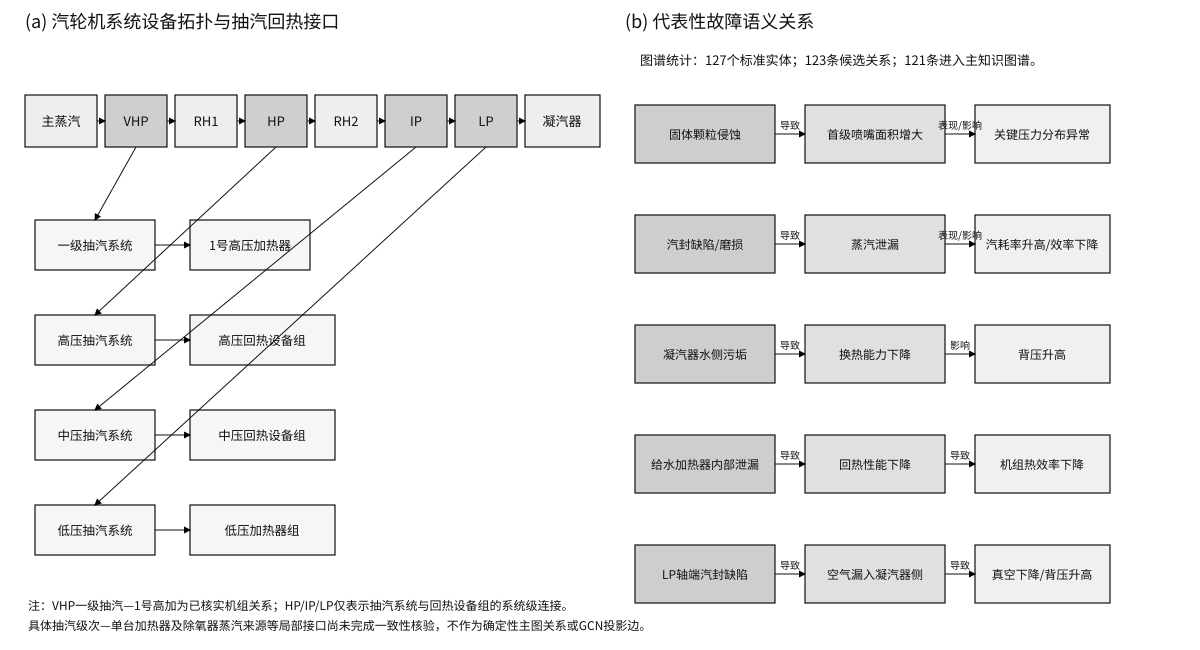
\includegraphics[width=0.99\textwidth]{figures/ch3/fig3_2_turbine_kg_overview.pdf}
      \caption{汽轮机系统知识图谱设备拓扑及代表性故障语义关系}
      \label{fig:turbine_kg_overview_final}
    \end{figure}
    图~\ref{fig:turbine_kg_overview_final}仅展示进入主知识图谱的可审计设备拓扑及代表性故障语义链路，用于说明系统结构与故障知识的组织方式；完整关系仍以审查后的知识三元组为准。存在资料差异的候选接口保持待核状态，不作为确定性图关系或后续GCN投影边。
  \fi
  \ThesisChThreeOriginalSubsection{#1}%
}
\renewcommand{\subsubsection}[1]{%
  \advance\ThesisChThreeSubsub by 1%
  \ifnum\ThesisChThreeSubsub=2
    \begin{figure}[htbp]
      \centering
      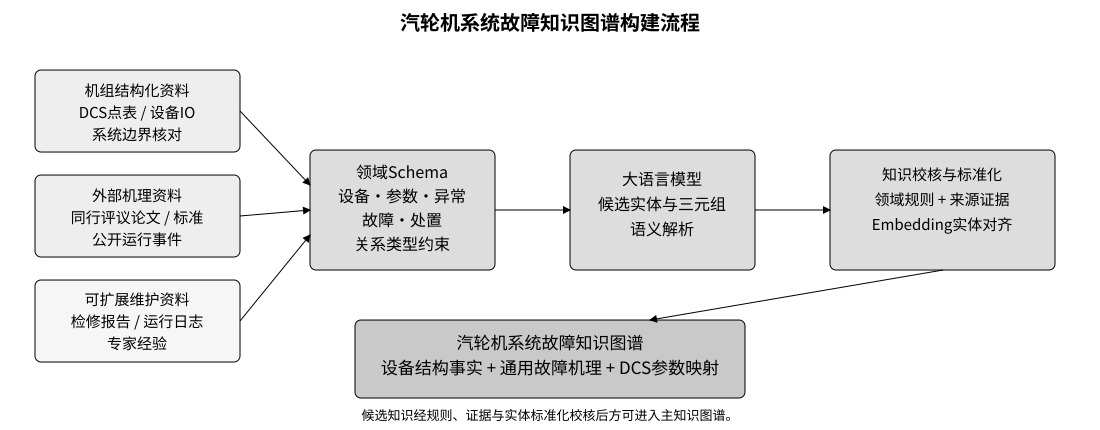
\includegraphics[width=0.98\textwidth]{figures/ch3/fig3_1_kg_construction_flow.pdf}
      \caption{汽轮机系统故障知识图谱构建流程}
      \label{fig:kg_construction_flow_final}
    \end{figure}
  \fi
  \ThesisChThreeOriginalSubsubsection{#1}%
}
\section{基于运行生产资料的汽轮机系统故障知识图谱构建}
\label{sec:knowledge_graph_v8}

\subsection{引言}

燃煤机组汽轮机系统由多级汽缸、再热系统、抽汽回热系统以及凝汽器冷端等多个热力设备组成，各设备通过蒸汽、凝结水和给水持续进行物质与能量传递。局部设备发生通流、汽封或换热性能异常后，其影响通常不会局限于单一监测参数，而会沿实际热力连接向相邻设备和参数传播。第二章建立的健康状态模型能够在给定运行边界下获得设备状态参数的健康参考值，并由实测值与模型输出之间的偏差信息表征状态变化程度。然而，仅依据参数偏差仍难以刻画参数所属设备、参数之间的物理联系以及多参数异常与故障机理之间的关联。

电站长期设计、运行和维护过程中积累了大量设备结构、DCS测点、系统接口、故障分析和检修经验等生产资料。这些知识既存在于点表、设备清单等结构化数据中，也分布于技术报告、标准和公开文献等文本资料中。知识图谱（Knowledge Graph，KG）能够以实体和关系组织多源异构知识，并利用图结构显式表示设备、参数、异常与故障之间的语义联系\cite{Hogan2021KnowledgeGraphs}。因此，将汽轮机运行生产资料转化为领域知识图谱，可以为后续图卷积故障诊断提供具有工程含义的结构先验。

本章首先分析汽轮机系统参数关联与典型故障特性，明确知识图谱需要描述的对象；随后整理机组DCS点表、设备输入输出关系和系统边界资料，并利用公开论文、标准及运行事件资料补充故障机理知识；在此基础上定义实体和关系类型，采用大语言模型生成候选三元组，并通过领域规则、来源证据和Embedding语义对齐完成知识校核与实体标准化。最终形成能够与实际DCS状态量建立映射的汽轮机系统故障知识图谱。

\subsection{燃煤机组汽轮机系统参数及故障特性}
\label{subsec:turbine_fault_characteristics_v8}

汽轮机主通流可概括为“主蒸汽--VHP--一次再热--HP--二次再热--IP--LP--凝汽器”。主蒸汽压力、温度和流量构成VHP入口热力边界，VHP排汽进入一次再热系统，一次热再蒸汽形成HP入口条件，HP排汽经二次再热后进入IP，最终蒸汽经LP膨胀后排入凝汽器。除主通流外，各级汽缸还通过抽汽支路向回热系统提供热源，使汽轮机本体与高压加热器、低压加热器、除氧器及给水系统形成进一步耦合。

根据已核对的机组资料，VHP一级抽汽与1号高压加热器相连。对于HP、IP和LP侧回热支路，现有资料能够确认其分别通过高压、中压和低压抽汽系统与相应回热设备形成系统级连接，但对具体抽汽级次与单台加热器的一一对应尚未完成机组级一致性核验；除氧器蒸汽来源等局部接口在不同资料中亦存在差异。因此，本文系统级知识图谱仅保留已核实的VHP一级抽汽--1号高压加热器关系，以及HP、IP、LP与相应抽汽/回热设备组之间的系统级连接，不将尚未核实的具体级次--单台设备关系作为确定性拓扑写入后续参数图。

汽轮机热力故障通常表现为多个状态参数的协同变化。Kubiak等针对汽轮机部件退化的案例研究表明，固体颗粒侵蚀会改变喷嘴或叶片有效通流面积，并影响关键压力分布\cite{Kubiak2002TurbineDegradation}。针对蒸汽轮机叶片沉积的跨型式研究进一步表明，沉积可减小有效通流面积，并可能降低出力和效率\cite{Kubiak2002ScaleDeposit}。该研究对象为地热蒸汽轮机，因此本文仅将其作为通用蒸汽轮机沉积机理参考，而不作为本文燃煤机组的现场直接证据。

汽封异常同样具有明显的结构传播特征。级间或轴端汽封缺陷会增加蒸汽泄漏，并影响汽轮机经济性；低压侧轴端密封异常还可能造成空气漏入和真空损失\cite{ZhangHu2021FaultPropagationGNN}。针对HP--IP中间汽封泄漏的研究表明，热再温度、IP排汽温度以及IP效率与该类泄漏具有诊断关联\cite{Xu2011HPIPLeakage}。上述关系反映的是设备层面和参数层面的通用机理，不直接规定本文VHP某一具体DCS测点的固定增减方向。

冷端和回热系统的故障也会沿热力接口影响汽轮机状态。燃煤机组凝汽器研究表明，水侧污垢会降低凝汽器换热有效性；凝汽压力还受到循环水温度、流量及换热状态等因素影响，并进一步影响机组热力性能\cite{Li2016CondenserFouling,Medica2018CondenserCondition}。给水加热器内部泄漏会破坏正常回热过程并影响循环效率，换热功率等过程指标可用于跟踪加热器慢性性能变化\cite{Heo2012FWHLeakage,Barszcz2011FeedwaterHeater}。

由上述过程可见，同一故障在多个参数上的响应受到设备归属和热力传播路径约束，而不同故障又可能共享部分压力、温度或流量参数。若仅依据局部数值相似性进行分类，容易产生故障类别混淆。因此，故障知识图谱需要同时表示设备连接、参数归属、故障发生位置、异常表现及处置关系，为多参数故障诊断提供结构化知识基础。

\subsection{基于运行生产资料的知识图谱构建方法}
\label{subsec:kg_construction_v8}

\subsubsection{汽轮机热力过程的运行生产资料}
\label{subsubsec:operation_materials_v8}

运行生产资料是领域故障知识图谱的主要知识来源。本文能够直接获得的机组资料包括DCS测点表、设备输入输出关系、系统边界核对结果以及状态监测建模资料。该类资料主要用于确定设备名称、参数点号、参数归属、主通流方向、抽汽支路及相邻设备接口，为设备实体、参数实体和机组拓扑关系提供事实依据。

现场结构资料难以完整覆盖典型故障的原因、演化过程和异常表现。为补充故障机理知识，本文进一步引入同行评议论文、标准、设备运行维护资料和公开运行事件报告。跨机组资料主要用于提取具有通用物理意义的“故障--异常--参数”关系，不直接将其他机组中某一具体测点的变化方向套用于本文机组。主要资料来源及用途见表~\ref{tab:kg_sources_v8}。

\begin{table}[htbp]
    \centering
    \caption{汽轮机故障知识图谱的主要知识来源}
    \label{tab:kg_sources_v8}
    \begin{tabular}{p{3.8cm}p{5.2cm}p{5.2cm}}
        \toprule
        资料类型 & 主要内容 & 图谱中的主要用途 \\
        \midrule
        DCS点表与设备IO资料 & 测点名称、点号、设备归属、入口和出口边界 & 构建设备、参数实体及机组直接拓扑 \\
        系统边界与状态建模资料 & 主通流、抽汽、再热及设备边界关系 & 校核设备接口和DCS映射 \\
        同行评议论文 & 汽封泄漏、通流侵蚀、沉积、冷端及回热故障机理 & 提取故障、异常和参数之间的通用关系 \\
        标准、维护资料及公开运行事件 & 故障现象、运行影响和处置经验 & 补充并交叉核验故障关系 \\
        \bottomrule
    \end{tabular}
\end{table}

在知识入图过程中，对机组结构事实与外部故障机理进行分层管理。由DCS、设备IO和系统拓扑直接确认的关系用于描述本文机组设备结构；由论文、标准或公开运行事件直接支持的关系用于描述通用故障机理；仅能依据热力规律推导而缺少直接证据的点级响应不作为主知识图谱中的确定关系。这样既保持机组拓扑与实际对象一致，也避免将跨机组经验过度外推至具体DCS测点。

\begin{figure}[htbp]
    \centering
    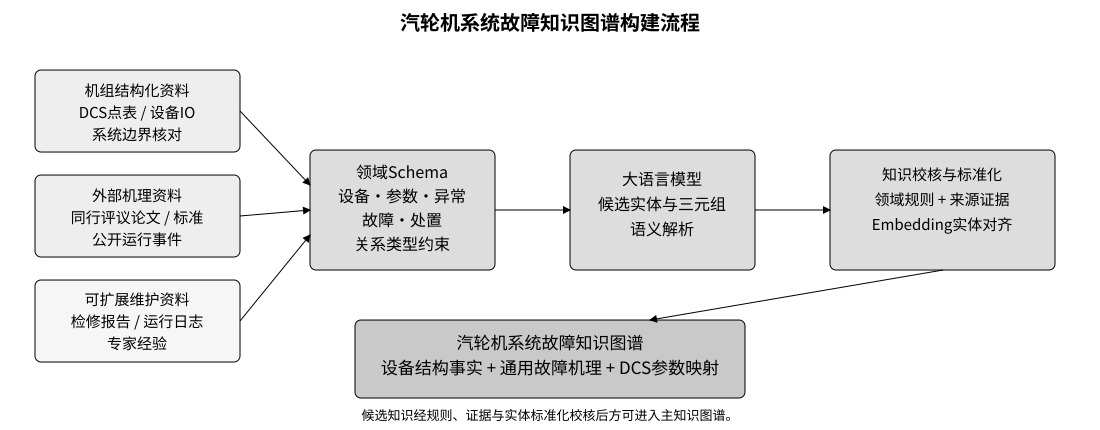
\includegraphics[width=0.98\textwidth]{figures/ch3/fig3_1_kg_construction_flow.pdf}
    \caption{汽轮机系统故障知识图谱构建流程}
    \label{fig:kg_construction_flow_v8}
\end{figure}

\subsubsection{节点和关系的构建与提取}
\label{subsubsec:entity_relation_v8}

运行生产资料中的设备、参数和故障信息通常以自然语言、工程简称或DCS编码等不同形式出现，同一对象在不同资料中可能存在多种表达。若缺少统一的实体和关系定义，知识抽取结果容易出现实体重复、语义边界不清以及关系方向混杂等问题。因此，首先需要建立适用于汽轮机故障诊断的知识图谱Schema。

设汽轮机系统故障知识图谱为
\begin{equation}
G_{KG}=(V,E,\mathcal R),
\end{equation}
式中：$V$为实体集合；$E$为实体间关系边集合；$\mathcal R$为关系类型集合。根据诊断任务需求，将实体划分为设备、参数、异常、故障和处置五类：
\begin{equation}
V=V_{dev}\cup V_{par}\cup V_{abn}\cup V_{fault}\cup V_{act}.
\end{equation}
设备实体表示VHP、HP、IP、LP、再热系统、抽汽支路、加热器和凝汽器等物理对象；参数实体表示可由DCS直接获取的压力、温度、流量和阀位等运行量；异常实体描述蒸汽泄漏、真空下降、通流面积变化和效率降低等状态现象；故障实体表示具有独立工程含义的故障类型；处置实体表示检查、清洗和检修等维护措施。

在实体类型确定后，根据汽轮机系统结构和故障语义定义设备归属、介质流向、设备接口、发生于、导致、表现为、影响、关联监测和处置为等关系。主要关系类型见表~\ref{tab:kg_relation_types_v8}。

\begin{table}[htbp]
    \centering
    \caption{汽轮机故障知识图谱主要关系类型}
    \label{tab:kg_relation_types_v8}
    \begin{tabular}{lll}
        \toprule
        关系类型 & 头实体类型 & 尾实体类型 \\
        \midrule
        归属 & 参数 & 设备 \\
        介质流向/设备接口 & 设备 & 设备 \\
        发生于 & 故障 & 设备 \\
        导致/表现为 & 故障或异常 & 异常 \\
        影响/关联监测 & 故障或异常 & 参数 \\
        处置为 & 故障 & 处置 \\
        \bottomrule
    \end{tabular}
\end{table}

完成Schema定义后，利用大语言模型对设备资料和故障文本进行语义解析，并按照预定义实体与关系类型输出候选三元组。语言模型能够快速识别文本中的设备、参数、异常、故障及处置对象，但其输出仅作为候选知识，不能直接写入最终图谱。

候选三元组首先经过领域规则校核。规则包括实体类型约束、关系方向约束、设备兼容性约束和参数可观测性约束。例如，“压力升高”“阀位异常”等带有状态方向的表达应归入异常实体，而不能作为实时数值参数节点；不存在于本文机组结构中的设备连接，也不能仅依据通用汽轮机结构建立为机组确定关系。通过规则校核可剔除类型错误、方向错误和设备不兼容的候选知识。

经过规则校核后，再对实体名称进行标准化。本文采用Embedding语义对齐处理设备简称、参数别名和不同文本写法\cite{Reimers2019SentenceBERT}。对于候选实体$v_i$和标准实体$v_j$，综合语义向量相似度和字符串相似度计算匹配程度：
\begin{equation}
S_{ij}=\lambda S_{emb}(v_i,v_j)+(1-\lambda)S_{str}(v_i,v_j),
\end{equation}
式中：$S_{emb}$为Embedding语义相似度；$S_{str}$为字符串相似度；$\lambda$为两类相似度的权重系数。当综合相似度达到设定阈值且实体类型一致时，将候选实体归并至标准实体；否则保留为待核对象。

最后，综合候选抽取、规则校核、实体标准化结果和来源证据评价关系可靠性。对于第$e$条候选关系，其置信度可表示为
\begin{equation}
C_e=\alpha C_{llm}+\beta C_{rule}+\gamma C_{emb}+\delta C_{evi},
\end{equation}
式中：$C_{llm}$为语言模型候选抽取置信度；$C_{rule}$为领域规则一致性得分；$C_{emb}$为实体语义对齐置信度；$C_{evi}$为来源证据强度；$\alpha$、$\beta$、$\gamma$和$\delta$为相应权重。机组设备连接关系以DCS和设备IO资料为优先依据，故障机理关系保留可追溯的论文、标准或运行事件来源。经过上述处理，分散于多源资料中的知识被统一表示为“头实体--关系--尾实体”三元组，并组成汽轮机系统故障知识图谱。

\subsection{知识图谱构建结果}
\label{subsec:kg_result_v8}

按照上述流程，形成了覆盖汽轮机主通流、再热、抽汽回热和凝汽冷端等对象的故障知识库。审查后的知识库共包含127个标准实体和123条候选关系。其中81条关系来自本文机组设备结构与DCS资料，40条关系由公开论文、标准或运行事件中的直接故障机理支撑；另有2条候选关系因不同机组资料之间存在描述差异而暂不纳入主知识图谱。因此，当前用于论文知识表达和后续参数图投影的主知识图谱包含121条可用关系。

在设备拓扑方面，图谱保存“主蒸汽--VHP--一次再热--HP--二次再热--IP--LP--凝汽器”的主通流关系，并包含VHP一级抽汽至1号高压加热器，以及HP、IP、LP与高压、中压、低压抽汽系统及相应回热设备组之间的系统级连接。对具体抽汽级次--单台加热器和除氧器蒸汽来源等尚存在资料差异的局部接口，保持待核状态，不进入确定性参数图。在故障语义方面，图谱进一步连接汽封缺陷、蒸汽泄漏、通流侵蚀、叶片沉积、凝汽器污垢和回热设备泄漏等故障与相应异常状态、关联参数及处置知识。

系统级知识图谱用于表达完整汽轮机故障领域知识，而图卷积模型需要加载可实时获取的数值特征。因此，在知识图谱构建完成后，进一步建立标准参数实体与实际DCS测点之间的映射。第五章VHP代表性算例从系统知识图谱中抽取VHP本体、一级抽汽支路和一次再热接口对应的状态参数节点，形成设备任务参数子图，并将第二章健康状态模型产生的动态偏差信息加载至对应参数节点，实现静态领域知识与动态运行数据之间的连接。

\begin{figure}[htbp]
    \centering
    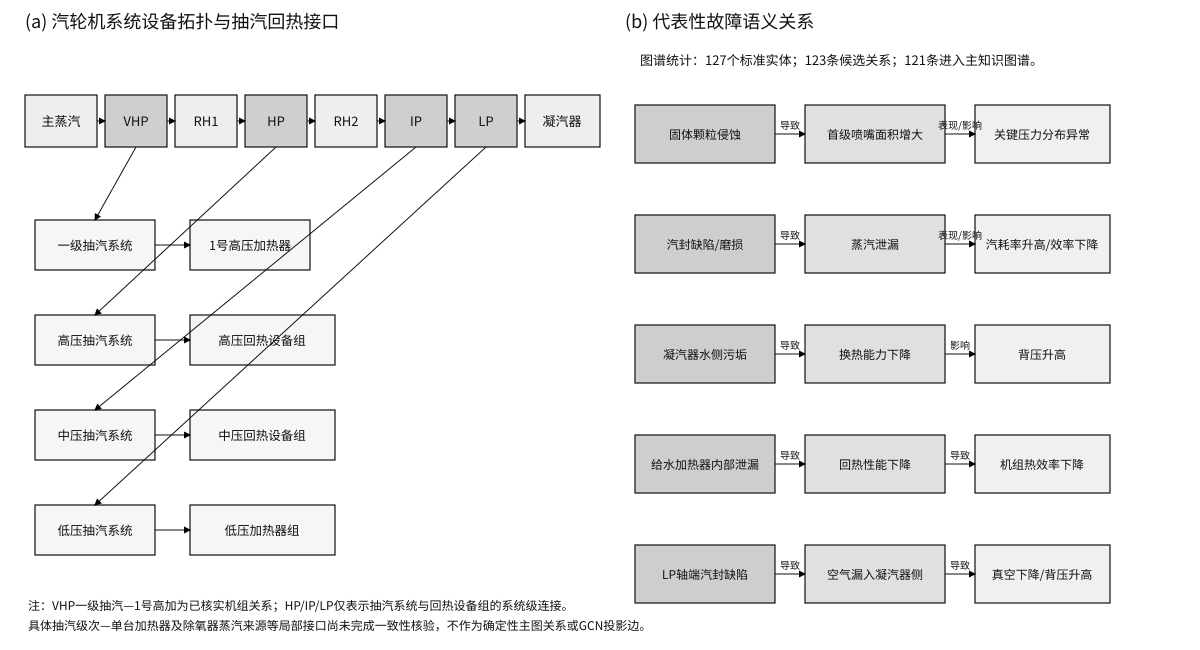
\includegraphics[width=0.99\textwidth]{figures/ch3/fig3_2_turbine_kg_overview.pdf}
    \caption{汽轮机系统知识图谱设备拓扑及代表性故障语义关系}
    \label{fig:turbine_kg_overview_v8}
\end{figure}

图~\ref{fig:turbine_kg_overview_v8}仅展示进入主知识图谱的可审计设备拓扑及代表性故障语义链路。VHP一级抽汽--1号高压加热器为已核实的机组直接关系；HP、IP和LP侧仅表示抽汽系统与相应回热设备组的系统级连接。具体抽汽级次--单台加热器以及除氧器蒸汽来源等尚未完成机组级一致性核验的局部接口，不作为确定性主图关系或后续GCN投影边。

\subsection{本章小结}

本章面向燃煤机组汽轮机系统构建了基于运行生产资料的故障知识图谱。首先分析汽轮机主通流、再热、抽汽回热和凝汽冷端之间的参数关联及典型热力故障的多参数传播特征；随后整理机组DCS点表、设备IO和系统边界资料，并利用公开论文、标准和运行事件补充故障机理知识；在此基础上定义设备、参数、异常、故障和处置等实体及相应关系类型，采用大语言模型生成候选三元组，并结合领域规则、来源证据和Embedding语义对齐完成知识校核与实体标准化。最终形成能够与实际DCS参数建立映射的汽轮机系统故障知识图谱，为下一章基于知识图谱和图卷积网络的故障诊断模型提供静态结构信息。
\endgroup

% Final wrapper for Chapter 4. The v7 text remains the method source of truth; this layer adds final figure placement and implementation-level clarifications verified against the frozen v07 training script.
\begingroup
\newcount\ThesisChFourSubsec
\ThesisChFourSubsec=0
\let\ThesisChFourOriginalSubsection\subsection
\renewcommand{\subsection}[1]{%
  \advance\ThesisChFourSubsec by 1%
  \ifnum\ThesisChFourSubsec=3
    \ThesisChFourOriginalSubsection{#1}%
    为统一全文术语，后文将实测状态与健康参考之间的差异统称为状态残差，其中$e_i(t)$表示原量纲状态残差，$r_i(t)$表示经训练集统计量标准化后的状态残差，$R_t$表示连续时间位置组成的多参数状态残差窗口。%
  \else
    \ifnum\ThesisChFourSubsec=4
      为与实际训练实现保持一致，两层GCN编码后并非直接对全部节点做全局平均。本文将节点初始表示$H^{(0)}$与第二层图卷积表示$H^{(2)}$在特征维拼接，并进行LayerNorm：
      \begin{equation}
      H_{cat}=\mathrm{LN}\left(H^{(0)}\Vert H^{(2)}\right)\in\mathbb R^{N\times 2d},
      \end{equation}
      式中，$\Vert$表示特征维拼接。分类阶段按照固定DCS节点顺序将$H_{cat}$展平为$2Nd$维向量，再依次通过96维全连接层、ReLU、Dropout(0.05)和故障类别输出层。该节点保持式读出既保留原始局部状态，又保留两层知识拓扑传播后的结构信息，避免全局平均池化消除固定测点的物理身份。预训练阶段则由线性解码器将每个节点的$2d$维表示恢复至长度为$L_r$的残差窗口，仅在被遮蔽位置计算重构误差。
      \begin{figure}[htbp]
        \centering
        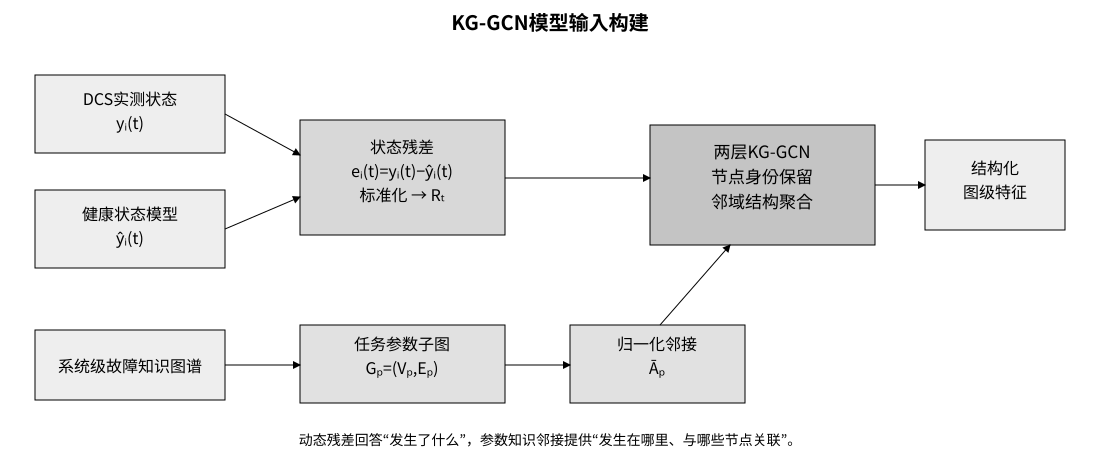
\includegraphics[width=0.98\textwidth]{figures/ch4/fig4_1_kg_gcn_input.pdf}
        \caption{KG-GCN模型输入构建过程}
        \label{fig:kg_gcn_input_final}
      \end{figure}
    \fi
    \ifnum\ThesisChFourSubsec=5
      \begin{figure}[htbp]
        \centering
        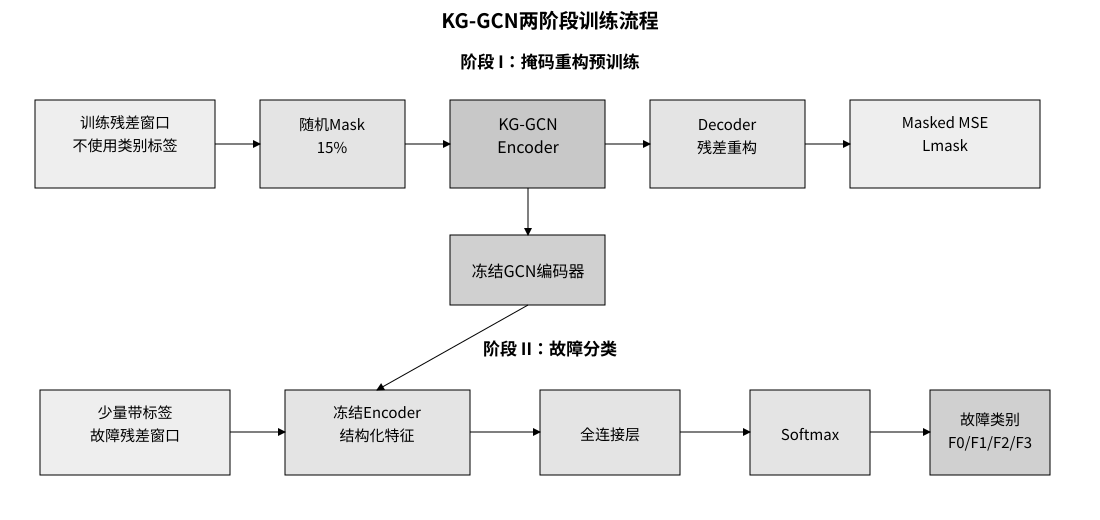
\includegraphics[width=0.98\textwidth]{figures/ch4/fig4_2_mask_training.pdf}
        \caption{KG-GCN掩码预训练与故障分类流程}
        \label{fig:mask_training_final}
      \end{figure}
    \fi
    \ThesisChFourOriginalSubsection{#1}%
  \fi
}
\section{基于KG-GCN的燃煤机组汽轮机系统故障诊断方法}
\label{sec:kg_gcn_v7}

\subsection{引言}

燃煤机组汽轮机系统故障具有多参数耦合和跨设备传播特征。传统阈值或经验规则方法依赖预先设定的异常判据，当运行边界变化或故障表现发生偏移时，其适应能力受到限制。纯数据驱动分类模型虽然能够学习复杂非线性特征，但通常将监测参数组织为规则向量或矩阵，参数之间的实际热力连接并未显式参与特征传播。当不同故障共享部分监测参数时，仅依赖局部数据特征容易出现类别混淆。

第三章构建的汽轮机系统故障知识图谱将设备、参数、异常和故障之间的关联组织为图结构，可为多参数诊断提供静态领域知识。第二章建立的健康状态模型则能够根据当前运行边界给出设备正常状态参考，并由实测状态与模型输出之间的偏差信息形成动态状态表征。本文将两类信息进行融合：以知识图谱投影得到的参数关系作为图结构，以状态监测偏差作为节点动态特征，通过GCN完成关联参数之间的信息聚合，并采用残差窗口遮蔽预训练提高少故障标签条件下的特征学习能力。

\subsection{图卷积网络}
\label{subsec:gcn_theory_v7}

汽轮机设备和参数之间构成由实际热力连接决定的非欧几里得拓扑。传统卷积运算依赖规则网格上的固定邻域，难以直接描述任意参数节点之间的连接关系。图卷积网络（Graph Convolutional Network，GCN）依据图邻接关系聚合节点自身及相邻节点特征，适合处理具有明确结构关系的工业过程数据\cite{Kipf2017GCN}。

设参数图为$G=(V,E)$，其中$V=\{v_1,v_2,\ldots,v_N\}$为参数节点集合，$E$为节点之间的关联边。图的拓扑由邻接矩阵$A\in\mathbb R^{N\times N}$表示。为使每次图卷积同时保留节点自身信息，在邻接矩阵中加入单位矩阵$I_N$：
\begin{equation}
\tilde A=A+I_N.
\end{equation}
式中，$\tilde A$为加入自连接后的邻接矩阵。相应度矩阵定义为
\begin{equation}
\tilde D_{ii}=\sum_j\tilde A_{ij}.
\end{equation}
在此基础上进行对称归一化，得到
\begin{equation}
\bar A=\tilde D^{-\frac{1}{2}}\tilde A\tilde D^{-\frac{1}{2}}.
\end{equation}
归一化处理可以减小不同节点度数差异对特征聚合幅值的影响。

设第$l$层节点特征矩阵为$H^{(l)}$，标准图卷积层的传播形式为
\begin{equation}
H^{(l+1)}=\sigma\left(\bar A H^{(l)}W^{(l)}\right),
\end{equation}
式中：$W^{(l)}$为第$l$层可学习权重矩阵；$\sigma(\cdot)$为非线性激活函数。每一层图卷积均按照邻接矩阵规定的连接路径，将目标节点及其邻域信息映射至新的特征空间。随着图卷积层数增加，节点能够逐步获得更远邻域内的关联信息。

本文采用两层GCN完成汽轮机参数关联信息聚合。考虑固定DCS参数自身状态同样具有诊断意义，在标准GCN基础上保留节点自身表示，并采用残差连接和LayerNorm抑制多层传播造成的局部信息衰减：
\begin{equation}
H^{(1)}=\mathrm{ReLU}\left[\mathrm{LN}\left(H^{(0)}+\bar A H^{(0)}W^{(1)}\right)\right],
\end{equation}
\begin{equation}
H^{(2)}=\mathrm{ReLU}\left[\mathrm{LN}\left(H^{(1)}+\bar A H^{(1)}W^{(2)}\right)\right].
\end{equation}
第一层聚合直接相邻参数信息，第二层进一步传递两跳邻域特征。由此，每个参数节点的表示同时包含自身动态变化和局部热力拓扑信息。

\subsection{KG-GCN模型输入构建}
\label{subsec:kg_input_v7}

第三章知识图谱包含设备、参数、异常、故障和处置等多种实体，而实时图卷积计算需要在参数节点上加载数值状态。因此，首先从系统级知识图谱中提取能够与实际DCS状态量建立映射的参数实体，并依据设备归属、介质流向和直接热力接口关系形成任务参数图。设任务参数图为
\begin{equation}
G_p=(V_p,E_p),
\end{equation}
式中：$V_p$为可加载实时状态的参数节点集合；$E_p$为由系统知识图谱投影得到的参数关联边。由$E_p$构建邻接矩阵$A_p$，并按前述方法得到归一化邻接矩阵$\bar A_p$。该矩阵在诊断过程中保持不变，用于规定不同参数之间的信息传播路径。

完成参数图构建后，将状态监测模型输出转化为动态节点特征。对于第$i$个状态参数，在时刻$t$的DCS实测值和健康状态模型输出分别记为$y_i(t)$和$\hat y_i(t)$，二者之间的状态偏差定义为
\begin{equation}
e_i(t)=y_i(t)-\hat y_i(t).
\end{equation}
在健康运行条件下，健康状态模型能够解释由负荷、入口边界和操作调节引起的大部分正常变化，$e_i(t)$主要反映预测误差和测量扰动；当设备状态发生异常时，实测状态相对于健康参考产生系统性偏离，相关参数的状态偏差随之发生变化。

由于不同参数的量纲和数值范围存在差异，对各参数状态偏差进行标准化：
\begin{equation}
r_i(t)=\frac{e_i(t)-\mu_i}{\sigma_i+\varepsilon},
\end{equation}
式中：$\mu_i$和$\sigma_i$分别为训练集第$i$个参数健康状态偏差的均值和标准差；$\varepsilon$为防止分母为零的微小常数。标准化统计量仅由训练数据计算，验证集和测试集不参与参数估计。

单一时刻全部参数的标准化状态偏差可写为
\begin{equation}
\mathbf r_t=[r_1(t),r_2(t),\ldots,r_N(t)]^{\mathrm T}.
\end{equation}
单时刻向量能够表示参数在当前时刻相对于健康参考的偏离，但无法描述故障随时间演化的连续特征。为此，对连续$L_r$个采样时刻进行滑动组织，构造参数--时间残差矩阵
\begin{equation}
R_t=
\begin{bmatrix}
r_1(t-L_r+1)&\cdots&r_1(t)\\
r_2(t-L_r+1)&\cdots&r_2(t)\\
\vdots&\ddots&\vdots\\
r_N(t-L_r+1)&\cdots&r_N(t)
\end{bmatrix}
\in\mathbb R^{N\times L_r}.
\end{equation}
式中，矩阵每一行固定对应一个参数节点，每一列对应一个连续时间位置。通过这种组织方式，多参数动态偏差被转化为能够与知识图谱节点一一对应的时序特征矩阵。

在GCN输入层中，首先将每个参数节点的时间窗口映射至$d$维初始特征空间：
\begin{equation}
H^{(0)}=\mathrm{ReLU}(R_tW_e+b_e),
\end{equation}
式中：$W_e\in\mathbb R^{L_r\times d}$和$b_e$分别为节点特征映射权重和偏置。随后，将节点初始特征$H^{(0)}$与知识图谱得到的归一化邻接矩阵$\bar A_p$共同输入GCN，实现动态运行信息在参数知识拓扑上的逐层传播。

固定DCS参数所在的物理位置本身具有诊断意义，因此本文在图级特征形成过程中保留节点顺序，不采用会完全消除节点身份的全局平均方式。最终图级特征同时包含节点局部状态和图卷积传播后的结构信息，并作为分类层输入。至此，知识图谱中的静态参数关系与状态监测模型产生的动态偏差信息被统一组织为KG-GCN的模型输入。

\subsection{KG-GCN模型训练}
\label{subsec:kg_training_v7}

故障类别标签通常需要依据运行记录、检修结论或人工确认获得，其获取成本明显高于一般运行状态数据。若直接使用有限的带标签故障样本训练全部图卷积参数，模型容易过度拟合已有故障模式。为减少对故障标签数量的依赖，本文采用两阶段训练方式：首先在不使用类别标签的残差窗口上进行掩码重构预训练，使GCN学习知识图谱约束下的参数关联；随后固定预训练后的图卷积编码器，仅利用带标签故障窗口训练分类层。

设预训练阶段使用的残差窗口集合为
\begin{equation}
\mathcal D_u=\{R^{(1)},R^{(2)},\ldots,R^{(M_u)}\},
\end{equation}
式中：$R^{(n)}$为第$n$个残差窗口；$M_u$为预训练窗口数量。预训练过程中随机遮蔽部分输入位置。设掩码矩阵为$M\in\{0,1\}^{N\times L_r}$，其中$M_{ij}=0$表示第$i$个参数在第$j$个时间位置被遮蔽，$M_{ij}=1$表示该位置保持可见，则遮蔽后的输入为
\begin{equation}
\tilde R=M\odot R+(1-M)\odot R_{mask}.
\end{equation}
式中：$\odot$表示逐元素乘法；$R_{mask}$表示遮蔽位置的替代值，本文取0。

将遮蔽后的残差窗口与参数邻接矩阵输入图卷积编码器：
\begin{equation}
Z=E_{\theta}(\bar A_p,\tilde R),
\end{equation}
式中：$E_{\theta}$为待预训练的GCN编码器；$\theta$为其中的可学习参数。编码器输出$Z$包含可见残差及其图邻域关联信息。随后通过解码器将结构化表示恢复至原始残差空间：
\begin{equation}
\hat R=D_{\phi}(Z),
\end{equation}
式中：$D_{\phi}$为解码器；$\phi$为解码器参数。

预训练阶段仅在被遮蔽位置计算重构误差：
\begin{equation}
\mathcal L_{mask}=\frac{\sum_{ij}(1-M_{ij})(R_{ij}-\hat R_{ij})^2}{\sum_{ij}(1-M_{ij})+\varepsilon}.
\end{equation}
通过最小化$\mathcal L_{mask}$，GCN编码器需要依据可见参数状态及其知识图谱邻域关系恢复缺失信息，从而在不使用故障类别标签的条件下学习多参数之间的结构化残差特征。

完成掩码预训练后，固定图卷积编码器参数，进入故障分类阶段。设带标签故障窗口样本集合为
\begin{equation}
\mathcal D_l=\{(R^{(n)},y^{(n)})\}_{n=1}^{M_l},
\end{equation}
式中：$R^{(n)}$为第$n$个故障残差窗口；$y^{(n)}$为对应故障类别标签；$M_l$为带标签故障样本数量。故障窗口经过预训练编码器后得到图级特征
\begin{equation}
\mathbf g^{(n)}=E_{\theta^*}(\bar A_p,R^{(n)}),
\end{equation}
式中：$\theta^*$表示预训练完成后固定的编码器参数。

分类层通过全连接映射和Softmax函数输出不同故障类别的预测概率：
\begin{equation}
\hat{\mathbf p}^{(n)}=\mathrm{Softmax}\left(W_c\mathbf g^{(n)}+b_c\right).
\end{equation}
式中：$W_c$和$b_c$分别为分类层权重和偏置。对于$C$类故障，分类阶段采用交叉熵损失函数
\begin{equation}
\mathcal L_{cls}=-\frac{1}{M_l}\sum_{n=1}^{M_l}\sum_{k=1}^{C}y_{nk}\log \hat p_{nk}.
\end{equation}
通过最小化$\mathcal L_{cls}$，分类层学习不同故障在图级残差特征空间中的判别边界。完成分类层训练后，新的残差窗口与参数邻接矩阵共同输入KG-GCN，即可获得相应故障类别概率。

\subsection{本章小结}

本章构建了基于知识图谱和图卷积网络的燃煤机组汽轮机系统故障诊断方法。首先介绍GCN在参数图上的特征传播过程，并采用两层图卷积聚合参数邻域信息；随后从第三章系统级知识图谱中抽取可与DCS状态量建立映射的参数关系，将第二章健康状态模型产生的多参数状态偏差组织为滑动时间窗口，与参数邻接矩阵共同形成KG-GCN输入；在模型训练阶段，首先在不使用类别标签的残差窗口上实施随机遮蔽重构预训练，随后固定图卷积编码器并利用带标签故障样本训练分类层。由此形成“知识图谱参数关系--状态监测偏差--图卷积特征传播--掩码预训练--故障分类”的诊断流程。下一章选取VHP作为代表性设备，对所提方法进行算例验证。
\endgroup

% Final Chapter 5 source. v8 integrates figures directly at the Yang-style result positions.
\section{故障诊断实验与结果分析}
\label{sec:experiments_v8}

\subsection{引言}

前述章节分别完成了汽轮机系统健康状态建模、故障知识图谱构建以及KG-GCN故障诊断模型设计。本章在此基础上开展算例验证。本文总体研究对象为燃煤机组汽轮机热力系统，第三章构建的系统级知识图谱覆盖主通流、再热、抽汽回热及凝汽器冷端等主要设备和参数关系。考虑当前数据完整性和实验基础，选取超高压缸（VHP）作为代表性设备，对所提出的汽轮机系统KG-GCN故障诊断方法进行验证。

实验采用真实健康运行残差作为正常状态背景，并依据独立故障机理构造具有不同空间作用区域和时间演化形式的半物理故障场景。在相同数据条件下分别训练CNN、AE和KG-GCN，通过Accuracy、Precision、Recall、F1以及混淆矩阵比较三种方法的故障识别性能。

\subsection{研究对象及故障数据集}
\label{subsec:fault_dataset_v8}

VHP位于主蒸汽进入汽轮机后的首个主要膨胀设备，其状态既受到主蒸汽压力、温度、流量和调节阀等入口边界影响，又通过排汽与一次再热系统相连，并通过一级抽汽支路向1号高压加热器提供抽汽。因此，在VHP局部范围内同时存在汽缸本体、一级抽汽支路和再热接口等不同物理区域，可用于观察不同故障在参数空间中的传播差异。

第二章VHP健康状态模型对设备状态参数进行同步预测。完成状态点筛选后，最终选取24个状态参数用于故障诊断，主要包括VHP叶片级压力、排汽压力与温度、一级抽汽口压力与温度、一级抽汽逆止门前后温度、1号高压加热器入口抽汽压力与温度、一次低温再热接口温度以及VHP缸壁和内部蒸汽温度等。每个状态参数均保持固定DCS身份，并通过第三章设备--参数映射关系对应至VHP任务参数子图。

结合汽轮机通流部件退化、汽封泄漏机理、一级抽汽支路结构以及24个状态参数的可观测范围，设置正常状态和三类典型故障场景，如表~\ref{tab:fault_classes_v8}所示。

\begin{table}[htbp]
    \centering
    \caption{VHP故障诊断样本类别}
    \label{tab:fault_classes_v8}
    \begin{tabular}{p{1.0cm}p{4.2cm}p{5.2cm}p{3.3cm}}
        \toprule
        类别 & 故障场景 & 主要状态特征 & 主要作用区域 \\
        \midrule
        F0 & 正常状态 & 真实健康运行残差，不叠加故障响应 & 全部诊断节点 \\
        F1 & VHP通流部件侵蚀 & 有效通流面积及级组压力分布发生改变 & VHP本体、排汽及再热接口 \\
        F2 & 一级抽汽支路泄漏 & 抽汽蒸汽损失并引起下游抽汽状态变化 & 一级抽汽及1号高加入口 \\
        F3 & VHP汽封泄漏 & 无效蒸汽泄漏引起本体及排汽热力状态改变 & VHP本体、排汽及相关接口 \\
        \bottomrule
    \end{tabular}
\end{table}

健康背景数据取自2024年6月独立运行数据。利用第二章GRU健康状态模型计算24个状态参数的实测值与健康预测值之差，形成真实健康残差背景。对于第$k$类故障，第$n$个故障残差窗口表示为
\begin{equation}
R_{k,n}^{F}=R_n^{H}+a_{k,n}S_k\odot G_{k,n}+\epsilon_{k,n},
\end{equation}
式中：$R_n^{H}$为真实健康残差窗口；$S_k$为依据独立故障机理确定的空间响应模式；$a_{k,n}$为故障严重程度系数；$G_{k,n}$为故障随时间演化的动态函数；$\epsilon_{k,n}$为小幅随机扰动。

为避免模型记忆单一固定故障模板，不同样本随机设置故障发生时刻，并采用阶跃、斜坡或Sigmoid等不同时间演化形式。主实验中故障扰动强度在训练健康残差标准差的$2.0\sim3.0\sigma$范围内随机变化，该参数用于描述构造场景中的相对异常强度，不对应设备实际损伤百分比。

数据划分在故障样本构造之前完成。每连续5个自然日中，第1--3日作为训练集，第4日作为验证集，第5日作为测试集，任一60~min窗口均不跨越自然日边界。按照上述规则，训练集、验证集和测试集分别包含1712、556和560个样本，各类别保持均衡，样本分布见表~\ref{tab:fault_split_v8}。

\begin{table}[htbp]
    \centering
    \caption{故障诊断数据集样本分布}
    \label{tab:fault_split_v8}
    \begin{tabular}{lrrrr}
        \toprule
        数据集 & F0 & F1 & F2 & F3 \\
        \midrule
        训练集 & 428 & 428 & 428 & 428 \\
        验证集 & 139 & 139 & 139 & 139 \\
        测试集 & 140 & 140 & 140 & 140 \\
        \bottomrule
    \end{tabular}
\end{table}

当前机组尚缺少能够覆盖上述多类故障的完整现场故障记录，因此本章样本属于基于真实健康残差和独立故障机理构造的半物理故障场景。相关实验用于检验所提方法在该类机理一致构造条件下的诊断性能。

\subsection{实验设置与评估指标}
\label{subsec:experiment_setting_v8}

为比较不同特征学习方式的诊断效果，选取CNN和AE作为主要对比算法。CNN将多参数残差窗口作为参数--时间二维矩阵，通过局部卷积核提取故障特征；AE首先通过无监督重构获得低维潜在表示，再利用分类层完成故障识别；KG-GCN将状态残差加载至知识图谱对应参数节点，并根据参数邻接关系进行图卷积特征传播。三种模型采用完全相同的训练集、验证集和测试集。

KG-GCN参数节点数量为24，残差窗口长度为60，图卷积编码器包含2层GCN，节点隐藏特征维数为32。预训练阶段随机遮蔽15\%的残差位置，通过重构被遮蔽残差训练GCN编码器；完成预训练后固定图卷积编码器参数，利用带标签故障窗口训练全连接分类层。优化器采用AdamW，权重衰减为$1\times10^{-4}$。主要实验参数见表~\ref{tab:kg_setting_v8}。

\begin{table}[htbp]
    \centering
    \caption{KG-GCN模型主要实验参数}
    \label{tab:kg_setting_v8}
    \begin{tabular}{ll}
        \toprule
        参数 & 取值 \\
        \midrule
        参数节点数量 & 24 \\
        残差窗口长度 & 60 \\
        GCN层数 & 2 \\
        节点隐藏特征维数 & 32 \\
        Mask比例 & 15\% \\
        分类层隐藏维数 & 96 \\
        优化器 & AdamW \\
        权重衰减 & $1\times10^{-4}$ \\
        \bottomrule
    \end{tabular}
\end{table}

本文采用Accuracy、Precision、Recall和F1-score评价不同模型的故障诊断性能。对于第$k$类故障，Precision和Recall分别定义为
\begin{equation}
P_k=\frac{TP_k}{TP_k+FP_k},
\end{equation}
\begin{equation}
R_k=\frac{TP_k}{TP_k+FN_k},
\end{equation}
式中：$TP_k$为第$k$类故障被正确识别的样本数量；$FP_k$为其他类别被误判为第$k$类故障的样本数量；$FN_k$为第$k$类故障被误判为其他类别的样本数量。相应F1值为
\begin{equation}
F1_k=\frac{2P_kR_k}{P_k+R_k}.
\end{equation}
在多分类条件下，本文对各类别Precision、Recall和F1进行宏平均。整体准确率定义为
\begin{equation}
Accuracy=\frac{N_{correct}}{N_{all}},
\end{equation}
式中：$N_{correct}$为正确分类样本数量；$N_{all}$为测试样本总数。除上述指标外，进一步利用混淆矩阵分析各故障类别的具体识别情况。

\subsection{诊断结果与对比}
\label{subsec:results_v8}

表~\ref{tab:main_result_v8}给出了CNN、AE和KG-GCN三种模型在固定随机种子123下的故障诊断结果。KG-GCN的Accuracy为98.57\%，高于CNN的97.86\%和AE的95.54\%；其宏平均Precision、Recall和F1分别为98.60\%、98.57\%和98.58\%，四项指标均为三种模型中的最高值。CNN的Accuracy和F1分别为97.86\%和97.85\%，整体诊断精度较高；AE的四项指标约为95.5\%，低于另外两种方法。

\begin{table}[htbp]
    \centering
    \caption{CNN、AE和KG-GCN诊断结果对比}
    \label{tab:main_result_v8}
    \begin{tabular}{lcccc}
        \toprule
        模型 & Accuracy/\% & Precision/\% & Recall/\% & F1/\% \\
        \midrule
        CNN & 97.86 & 97.89 & 97.86 & 97.85 \\
        AE & 95.54 & 95.57 & 95.54 & 95.54 \\
        \textbf{KG-GCN} & \textbf{98.57} & \textbf{98.60} & \textbf{98.57} & \textbf{98.58} \\
        \bottomrule
    \end{tabular}
\end{table}

为考察结果对随机初始化的敏感程度，采用3组随机种子重复训练。CNN、AE和KG-GCN的平均Macro-F1分别为98.33\%$\pm$0.45\%、96.43\%$\pm$0.82\%和98.46\%$\pm$0.11\%。KG-GCN平均F1最高，同时标准差最小，说明其在不同随机初始化条件下保持了较稳定的诊断结果。图~\ref{fig:main_comparison_v8}进一步给出了三种模型Macro-F1的均值及标准差。

\begin{figure}[htbp]
    \centering
    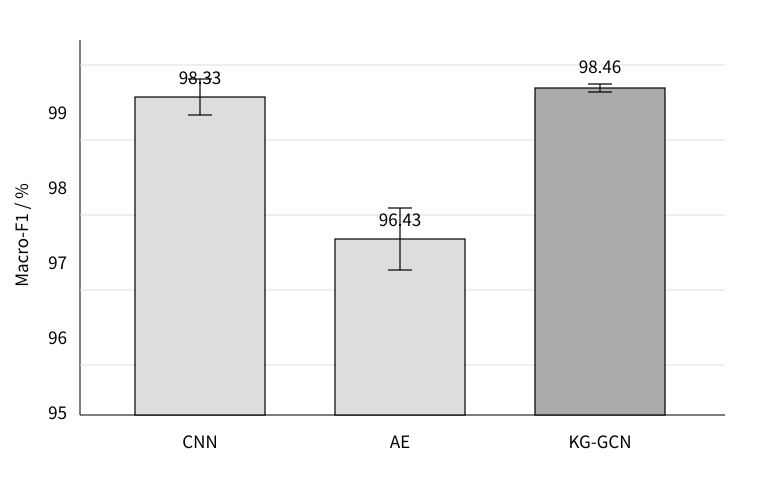
\includegraphics[width=0.78\textwidth]{figures/ch5/fig5_2_main_comparison.pdf}
    \caption{不同诊断模型三次重复实验Macro-F1比较}
    \label{fig:main_comparison_v8}
\end{figure}

为进一步观察各故障类别的误判方向，使用相同随机种子下的测试结果构造混淆矩阵，如图~\ref{fig:confusion_matrices_v8}所示。矩阵行表示真实类别，列表示预测类别。

\begin{figure}[htbp]
    \centering
    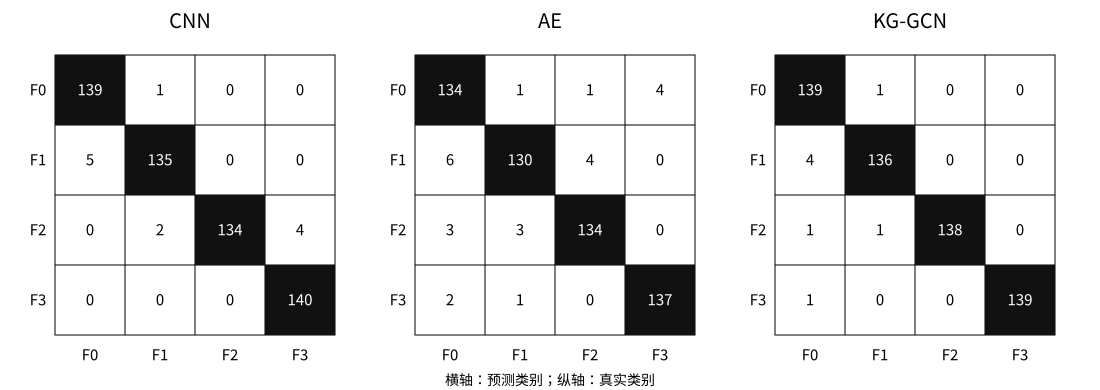
\includegraphics[width=0.99\textwidth]{figures/ch5/fig5_1_confusion_matrices.pdf}
    \caption{CNN、AE和KG-GCN故障诊断混淆矩阵}
    \label{fig:confusion_matrices_v8}
\end{figure}

由混淆矩阵可以看出，KG-GCN的分类结果最集中于主对角线，整体误诊数量最少。CNN共有12个测试样本发生误判，其中F2一级抽汽支路泄漏有4个样本被识别为F3 VHP汽封泄漏；AE共有25个样本发生误判，误判方向分散在F0、F1和F2等多个类别；KG-GCN仅有8个误判样本，其中F2有2个样本发生误判，F3仅有1个样本被识别为正常状态。

CNN主要依赖局部卷积核提取参数--时间矩阵中的局部动态特征。当不同故障在部分参数上的波动幅值或短时变化形态相近时，局部卷积特征难以显式表示这些参数在实际汽轮机结构中的位置差异。F2一级抽汽支路泄漏与F3 VHP汽封泄漏均可能在抽汽和排汽相关参数上形成状态变化，两类故障共享部分热力响应区域，因此CNN出现了F2向F3的类别交叉。

AE通过输入重构学习低维潜在表示，其优化目标主要描述多参数残差的整体数据分布。不同参数在潜在空间中的关联并不受到实际设备连接关系约束。当正常状态和不同故障的部分残差模式具有相近的重构特征时，分类层容易形成重叠的类别边界。由混淆矩阵可以看出，AE在多个类别之间均存在分散误判，与其总体F1低于CNN和KG-GCN的结果相对应。

KG-GCN在状态残差之外进一步利用了第三章知识图谱中的参数连接关系。对于F2故障，一级抽汽口、逆止门前后以及1号高压加热器入口构成连续的抽汽支路；对于VHP通流部件侵蚀和汽封泄漏，VHP本体压力、排汽状态以及一次再热接口形成不同的关联区域。GCN沿这些参数关系逐层聚合动态残差，使节点特征同时包含异常变化及其所在的热力结构位置。与只利用局部矩阵特征或潜在重构特征的模型相比，该结构信息有助于区分共享部分监测参数的故障类别，因此KG-GCN的混淆矩阵主对角线更加集中，整体误诊数量最低。

考虑故障标签数量有限时分类性能可能进一步下降，在主对比实验之后对掩码预训练进行补充验证。当分类阶段仅使用20\%带标签故障窗口时，直接从随机初始化训练KG-GCN的Macro-F1为94.48\%$\pm$0.93\%；采用残差窗口掩码预训练并固定GCN编码器后，Macro-F1提高至96.67\%$\pm$0.27\%，平均提高2.19个百分点。结果表明，在当前构造场景下，预训练能够利用不带类别标签的训练残差窗口提前学习参数之间的结构关联，并在故障标签减少时提供更稳定的特征表示。对应结果见图~\ref{fig:mask_ablation_v8}。

\begin{figure}[htbp]
    \centering
    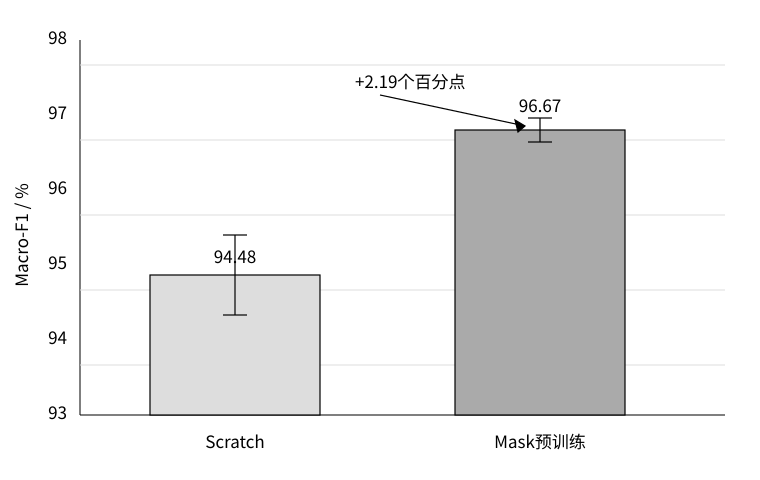
\includegraphics[width=0.76\textwidth]{figures/ch5/fig5_3_mask_ablation.pdf}
    \caption{20\%带标签样本下掩码预训练效果比较}
    \label{fig:mask_ablation_v8}
\end{figure}

\subsection{本章小结}

本章选取VHP作为代表性设备，对所提出的汽轮机系统KG-GCN故障诊断方法进行算例验证。基于2024年6月真实健康运行残差和独立故障机理构造正常状态、VHP通流部件侵蚀、一级抽汽支路泄漏和VHP汽封泄漏四类诊断样本，并按照自然日完成训练、验证和测试数据划分。在相同数据条件下，KG-GCN固定随机种子实验的Accuracy和F1分别达到98.57\%和98.58\%，均高于CNN和AE；混淆矩阵中KG-GCN的误诊样本数量最少。3组随机种子重复实验中，KG-GCN平均Macro-F1为98.46\%$\pm$0.11\%；在仅使用20\%带标签故障样本时，掩码预训练使Macro-F1提高2.19个百分点。上述结果说明，在本文构造的机理一致故障场景下，将状态监测残差信息与汽轮机参数知识关系进行融合，有助于提高多类别故障识别性能。当前结论仍需在后续现场故障记录或经校准的热力仿真数据上进一步验证。

\section{总结与展望}
\label{sec:conclusion_v2}

\subsection{论文主要工作}

本文以燃煤机组汽轮机热力系统为研究对象，针对宽负荷运行条件下正常状态基准难以确定、设备与故障知识分散以及高质量故障样本有限等问题，围绕设备健康状态建模、汽轮机故障知识图谱构建和KG-GCN故障诊断方法开展研究，形成了由动态运行数据与静态领域知识共同驱动的状态监测与故障诊断流程。主要研究工作和结论如下。

（1）针对汽轮机状态参数随负荷、蒸汽边界和运行调节持续变化的问题，建立了基于设备实际物理边界的GRU健康状态监测方法。按照$U+B\rightarrow Y$的设备级建模方式，将操作变量及上游/外部热力边界作为输入，以设备本体和热力接口状态作为输出，使模型学习给定运行条件下的正常响应关系。选取VHP作为代表性对象，利用2024年5月正常运行DCS数据训练，并采用2024年6月数据进行独立测试。ANN、TCN、iTransformer-small和GRU对比结果表明，GRU在最终24个状态参数上的宏平均$R^2$达到0.9511，在VHP本体、一级抽汽及一次冷再接口等主要状态上均获得较好的预测效果。由此建立的动态健康参考能够削弱正常工况变化对状态评价的干扰，并为后续利用实测值与健康预测值之间的偏差构造故障诊断动态特征提供基础。

（2）针对汽轮机设备连接关系复杂以及故障知识分散的问题，构建了基于运行生产资料的汽轮机系统故障知识图谱。结合本机DCS点表、设备输入输出关系和系统接口资料确定设备、参数及热力拓扑，并利用同行评议论文、标准和公开运行事件补充具有通用物理意义的故障机理。根据故障诊断需求定义设备、参数、异常、故障和处置等实体及相应关系类型，利用大语言模型完成候选三元组抽取，再结合实体类型、关系方向、设备兼容性、来源证据和Embedding语义对齐进行知识校核和实体标准化。当前审计知识库共包含127个标准实体和123条候选关系，其中121条关系进入主知识图谱，2条存在资料差异的候选关系保留待核。该知识图谱实现了汽轮机主通流、再热、抽汽回热和凝汽冷端等设备结构知识与故障机理知识的统一图结构表达。

（3）针对不同故障共享局部监测参数时容易产生类别混淆以及故障标签数量有限的问题，提出了基于知识图谱与图卷积网络的KG-GCN故障诊断方法。该方法首先将健康状态模型得到的多参数残差组织为滑动时间窗口，并映射为知识图谱参数节点的动态特征；随后将知识图谱投影得到的参数关系作为图结构输入，通过GCN沿设备和参数关联关系进行逐层特征聚合。训练阶段先在不使用类别标签的训练残差窗口上进行随机遮蔽重构预训练，再固定图卷积编码器并利用带标签故障窗口训练分类层。以VHP为代表性对象，基于真实健康运行残差与独立故障机理构造正常状态、VHP通流部件侵蚀、一级抽汽支路泄漏和VHP汽封泄漏四类半物理诊断场景。固定随机种子主实验中，KG-GCN的Accuracy和F1分别达到98.57\%和98.58\%，高于CNN和AE；3组随机种子重复实验的平均Macro-F1为98.46\%$\pm$0.11\%。在分类阶段仅使用20\%带标签故障窗口时，掩码预训练使Macro-F1由94.48\%提高至96.67\%，说明该训练方式能够在故障标签有限条件下改善模型诊断性能与结果稳定性。

综上，本文形成了“设备健康状态建模—状态残差构建—汽轮机故障知识图谱—图卷积结构化特征聚合—掩码预训练—故障分类”的完整技术流程。其中，知识图谱及KG-GCN方法面向燃煤机组汽轮机热力系统构建，VHP用于代表性算例验证。当前结果表明，健康状态残差能够为变工况下故障诊断提供统一动态表征，知识图谱能够为多参数残差提供实际热力结构约束，二者融合为汽轮机复杂故障诊断提供了一条数据与知识协同的技术路径。

\subsection{后续研究方向}

本文工作仍存在以下需要进一步研究的问题。

（1）\textbf{现场真实故障样本验证。} 当前故障分类实验采用真实健康运行残差背景，并依据独立故障机理构造半物理故障场景，能够用于验证模型在受控条件下的分类能力，但不能替代现场真实故障事件验证。后续应进一步收集机组缺陷记录、检修记录和历史故障数据，对不同故障的发生时刻、严重程度及多参数动态响应进行校准；在现场故障数据仍不足时，可结合经实际DCS数据校准的热力仿真模型补充不同故障程度和动态演化过程下的样本。

（2）\textbf{多设备及跨设备故障扩展。} 本文知识图谱覆盖汽轮机主通流、再热、抽汽回热及凝汽冷端等主要对象，但当前故障诊断算例仅对VHP任务子图进行了完整实验。后续可按照相同的设备级健康建模、参数节点映射和KG-GCN训练流程扩展至HP、IP、LP、凝汽器及回热设备，并进一步研究故障在相邻设备之间的传播、复合故障耦合以及系统级多故障并发识别问题。

（3）\textbf{知识图谱增量更新与不确定性建模。} 随着机组运行、检修和技术资料持续积累，汽轮机故障知识图谱需要具备增量更新能力。后续可建立面向运行日志、检修报告、技术通报和专家经验的候选知识抽取与审核机制，并进一步研究关系证据强度、边权重、动态图结构以及知识不确定性对GCN特征传播和故障诊断结果的影响，使领域知识能够随设备状态和运行经验持续更新。

（4）\textbf{复杂运行条件下的工程鲁棒性。} 实际在线应用还可能面临测点缺失、传感器漂移、工况分布变化和长期设备性能退化等问题。后续可将测点可靠性、缺失数据重构和在线分布漂移检测与KG-GCN诊断框架结合，并通过长期连续运行数据评价模型在不同季节、不同检修周期和不同负荷分布下的稳定性，为最终工程部署提供更加充分的验证依据。


% -------------------- 参考文献 --------------------
\printthesisbibliography

\end{document}
